\documentclass[abstracton,12pt,oneside]{scrreprt}

\usepackage[utf8]{inputenc}
\usepackage[T1]{fontenc}
\usepackage{fancyhdr}
\usepackage{graphicx}
\usepackage{tikz}
\usetikzlibrary{matrix}
\usepackage{times}
\usepackage{listings}
\usepackage{amssymb}
\usepackage{amsfonts}
%\usepackage{algorithm}
\usepackage{algpseudocode}
\usepackage{mathtools}
\usepackage{amsmath}
\usepackage[hyphens]{url}
\usepackage{chapterbib}
\usepackage{gensymb}
\usepackage{BTree}
\usepackage{weiwBTree}
\usepackage{float}
\usepackage{array}
\usetikzlibrary{shapes, calc}
\usepackage[ruled,linesnumbered,lined,commentsnumbered]{algorithm2e}
\usepackage{pgfplots}
\usepackage[titletoc]{appendix}
\usepackage{colortbl}


\expandafter\def\expandafter\UrlBreaks\expandafter{\UrlBreaks%  save the current one
	\do\a\do\b\do\c\do\d\do\e\do\f\do\g\do\h\do\i\do\j%
	\do\k\do\l\do\m\do\n\do\o\do\p\do\q\do\r\do\s\do\t%
	\do\u\do\v\do\w\do\x\do\y\do\z\do\A\do\B\do\C\do\D%
	\do\E\do\F\do\G\do\H\do\I\do\J\do\K\do\L\do\M\do\N%
	\do\O\do\P\do\Q\do\R\do\S\do\T\do\U\do\V\do\W\do\X%
	\do\Y\do\Z}

\DeclarePairedDelimiter\ceil{\lceil}{\rceil}
\DeclarePairedDelimiter\floor{\lfloor}{\rfloor}

\setlength{\parindent}{0pt} 


\titlehead{Department of Informatics, University of Zurich}
\subject{\vspace*{2cm}BSc Thesis}
\title{Implementing an Index Structure for Streaming Time Series Data}
\author{
  Melina Mast\\[-5pt]
  \scriptsize Matrikelnummer: 13-762-588\\[-5pt]
  \scriptsize Email: \texttt{melina.mast@uzh.ch}
}
\date{\vspace*{2cm}August, 2016}
\publishers{
  \small supervised by Prof.\ Dr.\ Michael Böhlen and Kevin Wellenzohn \\[5cm]
  \begin{tikzpicture}[overlay]
    \node at (-3,-3) {\includegraphics[height=5.5cm]{IFIlogo}};
    \node at (7,-3) {\includegraphics[height=2cm]{dbtgBW}};
  \end{tikzpicture}
}

%\dedication{dedicated to my family}

% --------- 

\newtheorem{definition}{Definition}
\newtheorem{example}{Example}
\newtheorem{theorem}{Theorem}
\newtheorem{lemma}{Lemma}

\newenvironment{proof}
  {\noindent{\bf Proof:\rm}}{\hfill$\Box$\vspace{\medskipamount}}

\def\bbbr{{\rm I\!R}}
\def\bbbm{{\rm I\!M}}
\def\bbbn{{\rm I\!N}}
\def\bbbz{{\rm I\!Z}}

% --------- 

\begin{document}


\maketitle

\chapter*{Acknowledgements}
I especially would like to thank my supervisor Kevin Wellenzohn for his advice, his amazing support and guidance. I could learn a lot from this thesis at the Database Technology Group of the University of Zurich. Therefore, I would like to thank Prof. Dr. Michael Böhlen for this opportunity. Besides, I would like to thank my boyfriend and my family for supporting me.


\begin{abstract}
A streaming time series is an unbounded sequence of data points that is continuously extended. The data points arrive in a predefined interval (e.g. every 5 minutes). Such time series are relevant to applications in diverse domains. Imagine a meteorology station that sends a temperature measurement every 3 minutes or imagine a trader in the financial stock market who receives updated pricing information every 5 minutes.\\
We present the implementation of an index structure for streaming time series data. The system keeps a limited amount of time series data in main memory. As a result, it is able to access the latest portion of past measurement data. We introduce an implementation using two data structures, a circular array and a $B^+$tree, to efficiently access the data of past measurements. The results of an experimental evaluation show the influence of the data structures on the system performance. 

\end{abstract}

\chapter*{Zusammenfassung}
Kontinuierliche Zeitreihen werden durch neu ankommende Daten stetig erweitert. Die Daten treffen dabei in einem vordefinierten Intervall ein.
Derartige Zeitreihen sind relevant für diverse Bereiche. Beispielsweise in der Meteorologie, in welcher die Wetterinformationen kontinuierlich aktualisiert werden oder, um einen weiteren Bereich zu nennen, in Finanzmärkten, wo die Händler auf die neusten Preisinformationen angewiesen sind.\\
Wir präsentieren die Implementation einer Indexstruktur für kontinuierlich erweiterte Zeitreihen. Unser System behält eine limitierte Anzahl der aktuellsten Daten im Arbeitsspeicher. Daraus resultiert, dass das System auf diese Daten zugreifen kann. Dazu stellen wir unsere Implementation vor, welche sich zwei Datenstrukturen zunutze macht: ein zirkuläres Array und ein $B^+$baum. Die beiden Datenstrukturen erlauben den effizienten Zugriff auf alle Werte der vergangenen Daten, welche sich in einem bestimmten Zeitfenster befinden. Die Resultate einer experimentellen Evaluation zeigen den Einfluss der Datenstrukturen auf die Laufzeit des Systems.

\tableofcontents
\listoffigures
\listoftables
\listofalgorithms
\renewcommand{\lstlistingname}{Algorithm}% Listing . Algorithm
\renewcommand{\listtablename}{Tables}

\addtocontents{loa}{\def\string\figurename{Algorithm}}

\newtheorem{defn}{Definition}
\newtheorem{exmp}{Example}[section]
\newcommand*{\argmin}{\operatornamewithlimits{argmin}\limits}

\chapter{Introduction}
A streaming time series is an unbounded sequence of data points that is continuously extended, potentially forever. The data points arrive in a predefined interval (e.g. every 5 minutes). Such time series are relevant to applications in diverse domains. For example, imagine a meteorology station that sends a temperature measurement every 3 minutes or, to name a different domain, imagine a trader in the financial stock market who depends on updated pricing information. Thus, various applications need to be fed continuously with the latest data. \\
But not only the current data can be interesting for an application. A streaming time series contains historical data that can be exploited. For example to recover missing values since a streaming time series is not always gapless. Due to sensor failures or transmission errors, values can get missing. To recover missing values the historical data can be utilised. Ideally, the missing value should be recovered efficiently, such that it is imputed before another new value arrive. Therefore, the efficient access of past time series data is important. \\
We present a system that keeps a limited size of data in main memory. The measurements with time points in a sliding time window are kept.  
\begin{defn}
	(Sliding Window) Let $W=[ \underline{t}, \bar{t} ]$ be a sliding window of length $|W|$. Time $\underline{t}$ represents the oldest time point that fits into the time window and time point $\bar{t}$ represents the most recent time point for which the stream produced a new value. 
\end{defn}
Because a portion of data is kept it is still accessible. The thesis proposes an implementation for an index structure for streaming time series data to efficiently access the time point and the value of measurements. In order to achieve efficient data access, the system uses two data structures: a circular array in combination with a $B^+$tree. 
The circular array has a size of length $|W|$. The measurements are stored in the array, sorted by time. The $B^+$tree as well contains the same measurements with time points in the sliding time window. The leaves of the tree are sorted from left to right by the measurement value. Thus, range queries can be efficiently performed. For every new measurement that the stream produces the time window slides forward. A value drops out of the window and a new value is inserted to the circular array and the $B^+$tree. Hence, if a measurement time point is not in the sliding window any more, it is removed from both data structures. \\
The described system is implemented and its advantages are outlined in this thesis. Furthermore, the system is analysed in terms of runtime and space complexity. Finally, an experimental evaluation tries to underpin the theoretical results.
\\ \\
At the beginning of this thesis, in Chapter \ref{background}, the TKCM algorithm is introduced. TKCM is designed by Wellenzohn et al.\cite{BScT}. The background aims to improve the understanding for the system context and for the requirements our system must satisfy. Chapter \ref{ProblemDefinition} describes the context and introduces the operations the system must be able to perform. In Chapter \ref{sec:Approach}, our approach is presented and its advantages are discussed. Further, the pseudo-code to implement the system is outlined. After that, the time and space complexity of the system is described in Chapter \ref{Complexity}. Followed by an experimental evaluation in Chapter \ref{sec:Experimental} to examine the theoretical results. Finally, the thesis is summed up in Chapter \ref{sec:Summary}.



\chapter{Background}
\label{background}
A streaming time series is not always gapless, but missing values can be recovered with the help of past data. To efficiently recover missing values, Wellenzohn et al.\cite{BScT} present the Top-$k$ Case Matching (TKCM) algorithm. The algorithm and its connection to this thesis is introduced in Section \ref{TKCM}.

\section{TKCM}
\label{TKCM}
TKCM recovers and imputes missing measurement values if it detects any. For each time series $s$ a set of correlated reference time series is determined to recover a missing value. Therefore, TKCM monitors a set of streaming time series and once a value is missing it defines a two-dimensional query pattern over the most recent values of a set of time series. The idea is to derive a missing value in time series $s$ from the \emph{k} most similar past pattern. 

\begin{defn}
	(Time Series) Let $S$ be a set $S = \{s_1,s_2,...\}$ of streaming time series. The measurement value of time series $s_i \in S$ at time $t$ is denoted as $s_i(t)$ and is represented by the tuple $(t,s_i(t))$. For a base time series $s$, let $R_s = \langle r_1, r_2,...\rangle$ be an ordered sequence of the time series $r_i \in S \setminus \{s\}$. The set of $\text{reference time series}$ for $s$, $R_s^d$, at the current time $\bar{t}$ are the first $d$ time series in $R_s$ for which $r(\bar{t}) \neq \text{NIL}$. The time points in a streaming time series $s$ are in time window $W$.
\end{defn}

TKCM retains a sliding window of the streaming time series in main memory.
To impute a missing value, TKCM defines a query pattern $Q(\bar{t})$ over the most recent values of the reference time series. Afterwards, TKCM searches for the \emph{k} most similar patterns in sliding window $W$.  
\begin{figure}[H]
	\centering
	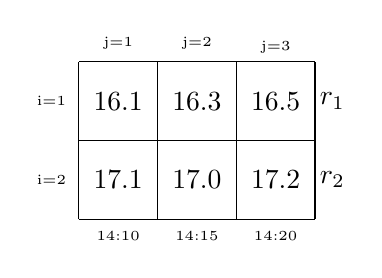
\begin{tikzpicture}
	\definecolor{mycolor}{RGB}{224,224,224}
	\definecolor{mycolor2}{RGB}{192,192,192}
	\draw[step=1cm,color=black] (0,0) grid (3,2);
	\node at (0.5,+0.5) [label={[font=\tiny,label distance=0.3cm]below:$\text{14:10}$}, label={[font=\tiny,label distance=0.1cm]left:$\text{i=2}$}]{17.1};
	\node at (1.5,+0.5) [label={[font=\tiny,label distance=0.3cm]below:$\text{14:15}$}]{17.0};
	\node at (2.5,+0.5) [label=right:$r_2$,label={[font=\tiny,label distance=0.3cm]below:$\text{14:20}$}]{17.2};
	\node at (0.5,+1.5) [label={[font=\tiny,label distance=0.3cm]above:$\text{j=1}$}, label={[font=\tiny,label distance=0.1cm]left:$\text{i=1}$}]{16.1};
	\node at (1.5,+1.5) [label={[font=\tiny,label distance=0.3cm]above:$\text{j=2}$}]{16.3};
	\node at (2.5,+1.5) [label=right:$r_1$,label={[font=\tiny,label distance=0.25cm]above:$\text{j=3}$}]{16.5};	
	\end{tikzpicture}
	\caption{Query pattern $Q(\bar{t})$ of length $l=3$ and $d=2$ reference time series at time point $\bar{t}=\text{14:20}$.} \label{QPat}
\end{figure}
\begin{defn}
	\label{pattCell}
	(Pattern) Let $R_s^d=\langle r_1,...,r_d \rangle$ be the sequence of reference time series for a time series $s$. A $pattern$ $P(t)$ of length $l > 0$ over $R_s^d$ that is embedded at time $t$ is defined as a $d\times l$ matrix $P(t) = [p_{i,j}]_{d\times l}$ where $p_{i,j}=S_i(t-l+j)$. We write $p_{i,j}\in P(t)$ to denote that value $p_{i,j}$ is contained in $P(t)$.
\end{defn}
The two-dimensional query pattern $Q(\bar{t})$ is anchored at time point $\bar{t}$ and consists the subsequence of length $l$ spanning from $\bar{t}-l+1$ to $\bar{t}$ of each reference time series. Each row represents a subsequence of a reference time series and each column represents the values of the reference time series at a time point as illustrated in Figure \ref{QPat}.\\ 
For every time point $t$ in $W$ exists a measurement which means $\forall t: \underline{t} \leq t < \bar{t} \rightarrow s(t) \ne \text{NIL}$ since \emph{s} contains imputed values if the real ones are missing. \\
TKCM  initializes one neighborhood $N(q_{i,j})$ around each $q_{i,j} \in Q(\bar{t})$. The algorithm looks for a new pattern $P(t)$ in time window $W$, such that $t \in W$, by \emph{growing} the neighborhood $N(q_{i,j})$ until the $k$ most similar patterns to $Q(\bar{t})$ have been found. TKCM stores the seen time points $t$ in a set $T$ to avoid considering these patterns again. 
\begin{defn}
		\label{def3}
	(Next Pattern) The next pattern for neighborhood $N(q_{i,j})$ is pattern $P(t) = [p_{i,j}]_{d\times l}$ anchored at time point $t = \argmin_{t \in W \setminus T} |p_{i,j}-q_{i,j}|$
\end{defn}
 To recover a missing value in a time series, past measurements need to be  accessed efficiently. Therefore, Wellenzohn et al.\cite{BScT} suggest a combination of two data structures: a $B^+$tree and a circular array. The necessary access methods are described in Section \ref{AccessMethods}.


\section{Access Methods}
\label{AccessMethods}
The next pattern (Def. \ref{def3}) is built on top of two access methods: sorted and random access. 
%check if follows or followed


\begin{defn}
	\label{sorted}
	(Sorted Access) Sorted access for a neighborhood $N(q_{i,j})$ returns the next yet unseen measurement $(t, s_i(t))$ where $t = \argmin_{t \in W \setminus T} |s_i(t) - q_{i,j}|$.
\end{defn}
\begin{defn}
	\label{random}
	(Random Access) Random access returns value $r(t)$, given time series $r$ and time point $t$.	
\end{defn}

Sorted access finds the most similar value to a given query pattern cell $q_{i,j}$ (Def. \ref{pattCell}), then, random access retrieves the values to fill the remaining pattern cells. \\
The next pattern search is presented in Algorithm \ref{NextPattern}. TKCM initializes a set $T =\{\}$. The set is filled during execution with all time points $t$ for which a pattern $P(t)$ has been processed. 
Using the sorted access mode, the algorithm finds the next yet unseen time point $t \notin T$ for which the value is most similar to a given query pattern value $q_{i,j}$. The random access mode is used to look up the values that pattern $P(t)$ is composed of. 


\begin{figure}[H]
	\centering
	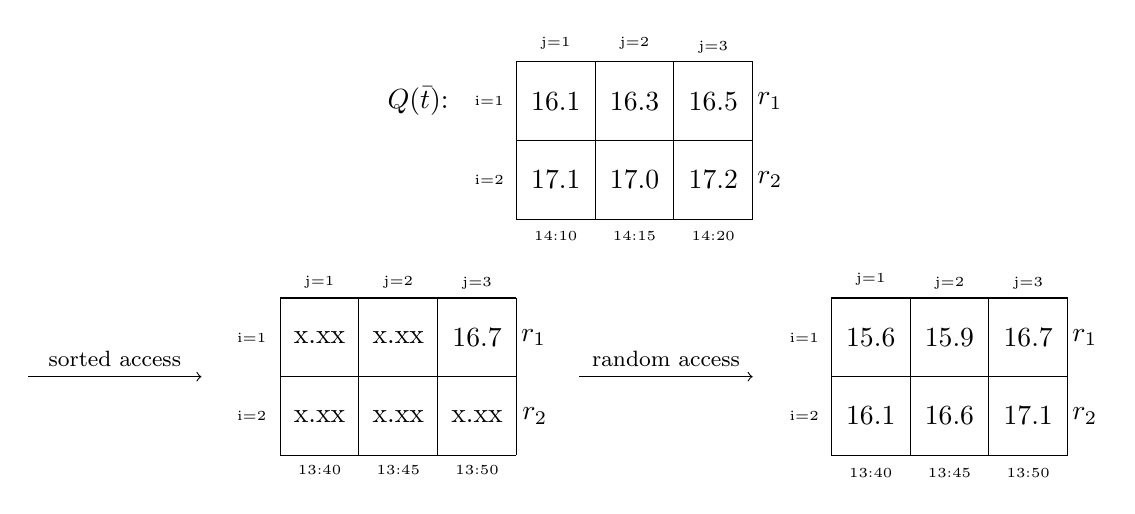
\begin{tikzpicture}
	\definecolor{mycolor}{RGB}{224,224,224}
	\definecolor{mycolor2}{RGB}{192,192,192}
		
	\draw[step=1cm,color=black] (3,3) grid (6,5);
	\node at (3.5,+3.5) [label={[font=\tiny,label distance=0.3cm]below:$\text{14:10}$}, label={[font=\tiny,label distance=0.1cm]left:$\text{i=2}$}]{17.1};
	\node at (4.5,+3.5) [label={[font=\tiny,label distance=0.3cm]below:$\text{14:15}$}]{17.0};
	\node at (5.5,+3.5) [label=right:$r_2$,label={[font=\tiny,label distance=0.3cm]below:$\text{14:20}$}]{17.2};
	\node at (3.5,+4.5) [label={[font=\tiny,label distance=0.3cm]above:$\text{j=1}$}, label={[font=\tiny,label distance=0.1cm]left:$\text{i=1}$}, label={[label distance=0.8cm]left:$Q(\bar{t})$:}]{16.1};
	\node at (4.5,+4.5) [label={[font=\tiny,label distance=0.3cm]above:$\text{j=2}$}]{16.3};
	\node at (5.5,+4.5) [label=right:$r_1$,label={[font=\tiny,label distance=0.25cm]above:$\text{j=3}$}]{16.5};	
	
	\definecolor{mycolor}{RGB}{224,224,224}
	\definecolor{mycolor2}{RGB}{192,192,192}
	
	\draw[->]  (-3.2,1) -- (-1,1) node [pos=0.5,above,font=\footnotesize] {sorted access};
	
	\draw[step=1cm,color=black] (0,0) grid (3,2);
	\node at (0.5,+0.5) [label={[font=\tiny,label distance=0.3cm]below:$\text{13:40}$}, label={[font=\tiny,label distance=0.1cm]left:$\text{i=2}$}]{x.xx};
	\node at (1.5,+0.5) [label={[font=\tiny,label distance=0.3cm]below:$\text{13:45}$}]{x.xx};
	\node at (2.5,+0.5) [label=right:$r_2$,label={[font=\tiny,label distance=0.3cm]below:$\text{13:50}$}]{x.xx};
	\node at (0.5,+1.5) [label={[font=\tiny,label distance=0.3cm]above:$\text{j=1}$}, label={[font=\tiny,label distance=0.1cm]left:$\text{i=1}$}]{x.xx};
	\node at (1.5,+1.5) [label={[font=\tiny,label distance=0.3cm]above:$\text{j=2}$}]{x.xx};
	\node at (2.5,+1.5) [label=right:$r_1$,label={[font=\tiny,label distance=0.25cm]above:$\text{j=3}$}]{16.7};
	
	\draw[->]  (3.8,1) -- (6.0,1) node [pos=0.5,above,font=\footnotesize] {random access};
	
	\draw[step=1cm,color=black] (7,0) grid (10,2);
	\node at (7.5,+0.5) [label={[font=\tiny,label distance=0.3cm]below:$\text{13:40}$}, label={[font=\tiny,label distance=0.1cm]left:$\text{i=2}$}]{16.1};
	\node at (8.5,+0.5) [label={[font=\tiny,label distance=0.3cm]below:$\text{13:45}$}]{16.6};
	\node at (9.5,+0.5) [label=right:$r_2$,label={[font=\tiny,label distance=0.3cm]below:$\text{13:50}$}]{17.1};
	\node at (7.5,+1.5)[label={[font=\tiny,label distance=0.3cm]above:$\text{j=1}$}, label={[font=\tiny,label distance=0.1cm]left:$\text{i=1}$}]{15.6};
	\node at (8.5,+1.5) [label={[font=\tiny,label distance=0.25cm]above:$\text{j=2}$}]{15.9};
	\node at (9.5,+1.5) [label=right:$r_1$,label={[font=\tiny,label distance=0.25cm]above:$\text{j=3}$}] {16.7} ;
	
	
	\end{tikzpicture}
	
	\caption{Pattern for query pattern cell $q_{1,3}$.}\label{fillQQ}
\end{figure}


\begin{table}
\centering
	\begin{tabular}{ | l | l | l | l|l|l|l|l|l|l|l|l|p{0.5cm} |}
		\hline
		Time t & 13:40 & 13:45 &13:50 & 13:55 & 14:00 & 14:05 & 14:10 & 14:15 & 14:20 \\ \hline
		$s(t)$ & 15.9 & 16.0 &16.3 &15.9 & 16.2 & 15.8 & 15.9 & 16.1 & x \\ \hline
		$r_1(t)$ & 15.6 & 15.9 &16.7 & 17.0 & 17.2& 16.2 & \cellcolor[gray]{0.9}16.1 & \cellcolor[gray]{0.9}16.3 & \cellcolor[gray]{0.9}16.5 \\ \hline
		$r_2(t)$ & 16.1 & 16.6 &17.1 & 15.2 & 16.0 & 15.4 & \cellcolor[gray]{0.9}17.1 & \cellcolor[gray]{0.9}17.0 & \cellcolor[gray]{0.9}17.2 \\ \hline
		
	\end{tabular}

 \caption{Data of the streaming time series $s$ and the reference time series $r_1$ and $r_2$}\label{table}
\end{table}


\begin{example}
	As illustrated in Table \ref{table} the value in time series $s$ at time point $\text{14:20}$ is missing. Therefore, a pattern is anchored at this time point. To find a pattern for pattern cell $q_{1,3}$ the next most similar value to $16.5$ is searched using sorted access as shown in Figure \ref{fillQQ}. This means, the difference between $16.5$ and $16.7$ is the smallest compared to other values in reference time series $r_1$. Then, the missing pattern values are filled. Therefore, the values in $r_1$ at time point $\text{13:40}$ and $\text{13:45}$ and the values in $r_2$ at $\text{13:40}$, $\text{13:45}$ and $\text{13:50}$ are inserted using random access. 
\end{example} 


\BlankLine
\begin{algorithm}[H]
	\IncMargin{1em}
	\SetAlgoLined
	\DontPrintSemicolon
	\KwIn{Neighborhood $N(q_{i,j})$ and seen time points $T$}
	\KwOut{Next pattern $P(t{'})$}

		P $\leftarrow$ matrix of size $d\times l$\;
		$(t, s_i(t))$ $\leftarrow$ sortedAccess(N($q_{i,j}$),$T$)\; 
		P[i,j] $\leftarrow$ $s_i(t)$\;	
		\ForEach{$q_{x,y}$ $ \in Q(\bar{t})$}
		{
		\If{$x \neq i$ {\bf and} $y\neq j$}{
			P[x,y] $\leftarrow$ randomAccess($s_x$, $t-j+y$)\;
		}
		}
		\Return P anchored at time $t-j+l$\;
	
	
	\caption{NextPattern($N(q_{i,j}),T$)}
	\label{NextPattern}
\end{algorithm}



\chapter{Problem Definition}
\label{ProblemDefinition}
The two access methods described in Section \ref{AccessMethods} are crucial for TKCM. However, they can be used in every application that needs access to past time series data. Therefore, the access methods should be usable for time series data in general. Hence, the data interval and the sliding window size should be variable. Furthermore, the access methods should be executable with duplicate values, since the measurements in time series data normally are not unique.
\\The present thesis introduces an implementation of the random and sorted access method for a streaming time series $s$. The required operations and the context for our system are presented in the following.

\section{Context}

We make the following assumptions for our system: 
\begin{itemize}  
	\item The measurements arrive in a predetermined interval (E.g. every five minutes). 
	\item There are no gaps between the measurements since gaps are filled before additional values are inserted to the data structure.
	\item No measurements arrive out-of-order.
\end{itemize}


\section{Operations}
\label{sec:Op}
The system needs to efficiently perform on the streaming time series $s$ in a sliding window $W$: 
\begin{itemize}  
	\item shift$(tree,array,\bar{t}, v)$: add value \emph{v} for the new current time point $\bar{t}$ and remove value \emph{v'} for the time point $\underline{t} - 1$ that just dropped out of time window $W$.
	\item sortedAccess$(N(q_{i,j}),T)$: given a neighborhood $N(q_{i,j})$ and a set of time points $T$, return the time point $t \not\in T$, as described in Definition \ref{sorted}.
	\item randomAccess$(array, t)$: return the value of time series \emph{s} at time \emph{t}, denoted by $s(t)$ (Def. \ref{random}).
	\item newNeighborhood$(tree,q_{i,j},t,j,l)$: given a value $q_{i,j} \in Q(\bar{t})$ for time point $t$, the pattern length $l$ and the index $j$, return the new neighborhood $N(q_{i,j})$.
\end{itemize}
The random access operation can be performed by the circular array, while the sorted access operation is executed on the leaves of a $B^+$tree. The thesis introduces an implementation of the random and sorted access method for a streaming time series $s$. The data structures and their advantages are described in Chapter \ref{sec:Approach}. Further, the thesis proposes a solution for handling duplicate values. 



\chapter{Approach}
\label{sec:Approach}
Each time series $s \in S$ is represented by a circular array. The circular array is kept in main memory. It uses random access to look up value $s(t)$ for a given time $t$. Further, for each time series $s$ a $B^+$tree is maintained that is also kept in main memory. The $B^+$tree is ideal for sorted access by value and therefore for range queries. Both data structures are described in detail in Section \ref{sec:circularArray} and Section \ref{sec:BplusTree}, respectively. Figure \ref{exampleTree} shows the data structures. All measurements in the circular array are represented in the $B^+$tree as well.

\begin{figure}[htbp]
	\centering
	\begin{tikzpicture}[
	scale=0.7,
	every node/.style={outer sep=0pt, transform shape, font=\scriptsize},
	every matrix/.style={cells={scale=0.7}},
	]
	% root node
	\xyshift{-20mm}{0mm}{\btreeinodethree{root}{17.1}{}{}};
	
	%
	% intermediate nodes
	\xyshift{-50mm}{-15mm}{\btreeinodethree{n1}{7.2}{}{}{}}
	\xyshift{ 10mm}{-15mm}{\btreeinodethree{n2}{23.0}{37.6}{43.1}}
	%
	% connecting root to intermediate level nodes
	\foreach \x in {1,2} { \btreelink{root-\x}{n\x} }
	%
	% leaf nodes
	\xyshift{-90mm}{-30mm}{\btreelnodethree{n11}{2.5}{3.0}{}}
	\xyshift{-60mm}{-30mm}{\btreelnodethree{n12}{7.2}{13.2}{}}
	\xyshift{-30mm}{-30mm}{\btreelnodethree{n21}{17.1}{18.1}{}}
	\xyshift{ 0mm}{-30mm}{\btreelnodethree{n22}{23.0}{25.4}{}}
	\xyshift{ 30mm}{-30mm}{\btreelnodethree{n23}{37.6}{38.9}{40.3}}
	\xyshift{ 60mm}{-30mm}{\btreelnodethree{n24}{43.1}{47.1}{}}
	%
	% connecting intermediate level to leaf nodes
	\foreach \x in {1,2}     { \btreelink{n1-\x}{n1\x} }
	\foreach \x in {1,2,3,4} { \btreelink{n2-\x}{n2\x} }
	%
	% leaf pointers
	\draw[btlink] ([yshift=+3pt] n11-c.east) -- ([yshift=+3pt] n12-a.west);
	\draw[btlink] ([yshift=-3pt] n12-a.west) -- ([yshift=-3pt] n11-c.east);
	\draw[btlink] ([yshift=+3pt] n12-c.east) -- ([yshift=+3pt] n21-a.west);
	\draw[btlink] ([yshift=-3pt] n21-a.west) -- ([yshift=-3pt] n12-c.east);
	\draw[btlink] ([yshift=+3pt] n21-c.east) -- ([yshift=+3pt] n22-a.west);
	\draw[btlink] ([yshift=-3pt] n22-a.west) -- ([yshift=-3pt] n21-c.east);
	\draw[btlink] ([yshift=+3pt] n22-c.east) -- ([yshift=+3pt] n23-a.west);
	\draw[btlink] ([yshift=-3pt] n23-a.west) -- ([yshift=-3pt] n22-c.east);
	\draw[btlink] ([yshift=+3pt] n23-c.east) -- ([yshift=+3pt] n24-a.west);
	\draw[btlink] ([yshift=-3pt] n24-a.west) -- ([yshift=-3pt] n23-c.east);
	%
	
	% circular array
	\xyshift{-40mm}{-50mm}{
		\matrix [ampersand replacement=\&, outer sep=0pt, matrix anchor=north] (array) {
			\node[circularptr] (c1)  {}; \\	
			%
			\node[circularval] (left)(right) {13:45}; \\
		};
	}
	% circular array
	\xyshift{-10mm}{-50mm}{
		\matrix [ampersand replacement=\&, outer sep=0pt, matrix anchor=north] (array) {
			\node[circularptr] (c2)  {}; \\	
			%
			\node[circularval] (left)(right) {14:15}; \\
		};
	}	
	
	% draw pointers between circular array and B+ tree
	\path[btlink2] ([yshift=-2pt] c1.center)  edge[out=90,in=270] ([yshift=2pt] n22-2.center);
	% draw pointers for linked list
	\draw[btlink] ([yshift=-10pt] c1.east) -- ([yshift=-10pt] c2.west);
	%\draw[btlink] ([yshift=-10pt] c2.east) -- ([yshift=-10pt] c1.east);
	\draw[btlink] ([yshift=-20pt] c2.west) -- ([yshift=-20pt] c1.east);
	
	%circular links
	\path[btlink] ([yshift=-10pt] c1.west)  edge[out=220,in=250] ([yshift=-10pt] c2.east);
	\path[btlink2] ([yshift=-20pt] c1.west)  edge[out=220,in=250] ([yshift=-20pt] c2.east);
	
	
	% list  value
	\xyshift{-90mm}{-50mm}{
		\matrix [ampersand replacement=\&, outer sep=0pt, matrix anchor=north] (array) {
			\node[circularptr] (c3)  {}; \\	
			%
			\node[circularval] (left)(right) {14:10}; \\
		};
	}
	
	% draw pointers between list value and B+ tree
	\path[btlink2] ([yshift=-2pt] c3.center)  edge[out=90,in=270] ([yshift=2pt] n11-1.center);
	
	%circular links
	\path[btlink] ([yshift=-16pt] c3.west)  edge[out=-1500,in=-60] ([yshift=-16pt] c3.east);
	\path[btlink2] ([yshift=-24pt] c3.west)  edge[out=-1500,in=-60] ([yshift=-24pt] c3.east);
		
	% list  value
	\xyshift{-60mm}{-50mm}{
		\matrix [ampersand replacement=\&, outer sep=0pt, matrix anchor=north] (array) {
			\node[circularptr] (c4)  {}; \\	
			%
			\node[circularval] (left)(right) {13:15}; \\
		};
	}
	
	
		% list  value
		\xyshift{05mm}{-50mm}{
			\matrix [ampersand replacement=\&, outer sep=0pt, matrix anchor=north] (array) {
				\node[circularptr] (c5)  {}; \\	
				%
				\node[circularval] (left)(right) {13:30}; \\
			};
		}
		
			% list  value
			\xyshift{20mm}{-50mm}{
				\matrix [ampersand replacement=\&, outer sep=0pt, matrix anchor=north] (array) {
					\node[circularptr] (c6)  {}; \\	
					%
					\node[circularval] (left)(right) {13:50}; \\
				};
			}
					% list  value
					\xyshift{40mm}{-50mm}{
						\matrix [ampersand replacement=\&, outer sep=0pt, matrix anchor=north] (array) {
							\node[circularptr] (c7)  {}; \\	
							%
							\node[circularval] (left)(right) {14:05}; \\
						};
					}
					
			
						% list  value
						\xyshift{60mm}{-50mm}{
							\matrix [ampersand replacement=\&, outer sep=0pt, matrix anchor=north] (array) {
								\node[circularptr] (c8)  {}; \\	
								%
								\node[circularval] (left)(right) {14:00}; \\
							};
						}
						
						% list  value
						\xyshift{80mm}{-50mm}{
							\matrix [ampersand replacement=\&, outer sep=0pt, matrix anchor=north] (array) {
								\node[circularptr] (c9)  {}; \\	
								%
								\node[circularval] (left)(right) {13:55}; \\
							};
						}
	
	% draw pointers between list value and B+ tree
	\path[btlink2] ([yshift=-2pt] c4.center)  edge[out=90,in=270] ([yshift=2pt] n12-2.center);
	
	%circular links
	\path[btlink] ([yshift=-16pt] c4.west)  edge[out=-1500,in=-60] ([yshift=-16pt] c4.east);
	\path[btlink2] ([yshift=-24pt] c4.west)  edge[out=-1500,in=-60] ([yshift=-24pt] c4.east);
	
		% draw pointers between list value and B+ tree
		\path[btlink2] ([yshift=-2pt] c5.center)  edge[out=90,in=270] ([yshift=2pt] n23-1.center);
		
		%circular links
		\path[btlink] ([yshift=-16pt] c5.west)  edge[out=-1500,in=-60] ([yshift=-16pt] c5.east);
		\path[btlink2] ([yshift=-24pt] c5.west)  edge[out=-1500,in=-60] ([yshift=-24pt] c5.east);
		
		
			% draw pointers between list value and B+ tree
			\path[btlink2] ([yshift=-2pt] c6.center)  edge[out=90,in=270] ([yshift=2pt] n23-2.center);
			\path[btlink2] ([yshift=-2pt] c7.center)  edge[out=90,in=270] ([yshift=2pt] n23-3.center);
			\path[btlink2] ([yshift=-2pt] c8.center)  edge[out=90,in=270] ([yshift=2pt] n24-1.center);
			\path[btlink2] ([yshift=-2pt] c9.center)  edge[out=90,in=270] ([yshift=2pt]n24-2.center);
			
			%circular links
			\path[btlink] ([yshift=-16pt] c6.west)  edge[out=-1500,in=-60] ([yshift=-16pt] c6.east);
			\path[btlink2] ([yshift=-24pt] c6.west)  edge[out=-1500,in=-60] ([yshift=-24pt] c6.east);
	
		%circular links
		\path[btlink] ([yshift=-16pt] c7.west)  edge[out=-1500,in=-60] ([yshift=-16pt] c7.east);
		\path[btlink2] ([yshift=-24pt] c7.west)  edge[out=-1500,in=-60] ([yshift=-24pt] c7.east);

		%circular links
		\path[btlink] ([yshift=-16pt] c8.west)  edge[out=-1500,in=-60] ([yshift=-16pt] c8.east);
		\path[btlink2] ([yshift=-24pt] c8.west)  edge[out=-1500,in=-60] ([yshift=-24pt] c8.east);
	
			%circular links
			\path[btlink] ([yshift=-16pt] c9.west)  edge[out=-1500,in=-60] ([yshift=-16pt] c9.east);
			\path[btlink2] ([yshift=-24pt] c9.west)  edge[out=-1500,in=-60] ([yshift=-24pt] c9.east);
	
	\foreach \x in
	{n11-2, n12-1,n21-1,n21-2,n22-1}
	{ \path[<-] ([yshift=-15pt] \x.center) edge ([yshift=2pt] \x.center); }
	
	
	\definecolor{mycolor}{RGB}{224,224,224}
	
	% circular array
	\xyshift{-15mm}{-80mm}{
		\matrix [ampersand replacement=\&, outer sep=0pt, matrix anchor=north] (array) {
			\node[circularptr] (c1)  {2.5}; \&
			\node[circularptr] (c2)  {25.4}; \&
			\draw node [black,midway,yshift=0.6cm] {lastPos};
			\node[circularptr, fill=mycolor] (c3)  {3.0}; \&
			\node[circularptr] (c4)  {13.2}; \&
			\node[circularptr] (c5)  {23.0}; \&
			\node[circularptr] (c6)  {17.1}; \&
			\node[circularptr] (c7)  {37.6}; \&
			\node[circularptr] (c8)  {18.1}; \&
			\node[circularptr] (c9)  {7.2}; \&
			\node[circularptr] (c10) {25.4}; \&
			\node[circularptr] (c11) {38.9}; \&
			\node[circularptr] (c12) {47.1}; \&
			\node[circularptr] (c13) {43.1}; \&
			\node[circularptr] (c14) {40.3};  \\
			%
			\node[circularval] (left) {14:10}; \&
			\node[circularval] {14:15}; \&
			\node[circularval, fill=mycolor] {14:20}; \&
			\node[circularval] {13:15}; \&
			\node[circularval] {13:20}; \&
			\node[circularval] {13:25}; \&
			\node[circularval] {13:30}; \&
			\node[circularval] {13:35}; \&
			\node[circularval] {13:40}; \&
			\node[circularval] {13:45}; \&
			\node[circularval] {13:50}; \&
			\node[circularval] {13:55}; \&
			\node[circularval] {14:00}; \&
			\node[circularval] (right){14:05};\\
		};
	}
	% curly brace
	\draw [decorate,decoration={brace,mirror,amplitude=10pt}]
	([yshift=-5pt] left.south west) -- ([yshift=-5pt] right.south east)
	node [black,midway,yshift=-0.9cm] {\large size $|W|$};

	
	\end{tikzpicture}
	\vspace{2mm}
	
	\caption{A $B^+$tree with the related circular array.}
	\label{exampleTree}
	
\end{figure}

\section{Circular Array}
\label{sec:circularArray}
A circular array is used to store the time series data sorted by time in the predefined window $W$. The value and the time point of a measurement is directly stored in the circular array. 
The size of the array is determined by $|W|$ and represents the capacity of the array. Hence, an array with $|W|=10$ can hold $10$ measurements. The last update position $lastPos$ is stored in a variable and is updated with every insertion. In detail, a circular array contains the following attributes: a counter $count$ that counts the number of measurements in the array, a $lastPos$ to store the position that was last updated with a measurement and finally the data, which actually holds the time points and values of the measurements.

\lstset{language=C}
\begin{lstlisting}
struct Measurement{
  timeStamp time;
  double value;
};

struct CircularArray{
  Measurement * data;
  int lastPos;
  int count;
};
\end{lstlisting}
\BlankLine

\subsection{States}
The circular array can be in two different states:
\begin{enumerate}  
	\item First, the array is filled with every new arriving measurement until every position in the circular array is occupied in array $1$ in Figure \ref{fig:cat},.  
	\item Afterwards, if all spaces in the circular array are occupied, the number of measurements stays constant because a value drops out if a new value is inserted to array $2$. 
\end{enumerate}

\begin{figure}[H]
	\centering
	\begin{tikzpicture}[
	scale=0.7,
	every node/.style={outer sep=0pt, transform shape, font=\scriptsize},
	every matrix/.style={cells={scale=0.7}},
	]
	
	\definecolor{mycolor}{RGB}{224,224,224}
	
	% circular array
	\xyshift{-15mm}{-70mm}{
		\matrix [ampersand replacement=\&, outer sep=0pt, matrix anchor=north] (array) {
			\draw node [black,midway,yshift=1cm, xshift=-1cm] {1.};
			\node[circularptr] (c1)  {2.2}; \&
			\node[circularptr] (c2)  {1.9}; \&
			\node[circularptr] (c3)  {1.5}; \&
			\node[circularptr] (c4)  {3.6}; \&
			\node[circularptr] (c5)  {6.2}; \&
			\draw node [black,midway,yshift=0.6cm] {lastPos};
			\node[circularptr, fill=mycolor] (c6)  {3.2}; \&
			\node[circularptr] (c7)  {}; \&
			\node[circularptr] (c8)  {}; \&
			\node[circularptr] (c9)  {}; \&
			\node[circularptr] (c10) {}; \&
			\node[circularptr] (c11) {}; \&
			\node[circularptr] (c12) {};  \\
			%
			\node[circularval] (left) {13:10}; \&
			\node[circularval] {13:15}; \&
			\node[circularval] {13:20}; \&
			\node[circularval] {13:25}; \&
			\node[circularval] {13:30}; \&
			\node[circularval, fill=mycolor] {13:35}; \&
			\node[circularval] {}; \&
			\node[circularval] {}; \&
			\node[circularval] {}; \&
			\node[circularval] {}; \&
			\node[circularval] {}; \&
			\node[circularval] (right){};\\
		};
	}
	
	% circular array
	\xyshift{-15mm}{-100mm}{
		\matrix [ampersand replacement=\&, outer sep=0pt, matrix anchor=north] (array) {
			\draw node [black,midway,yshift=1cm, xshift=-1cm] {2.};
			\node[circularptr] (c1)  {3.2}; \&
			\node[circularptr] (c2)  {1.3}; \&
			\node[circularptr] (c3)  {4.5}; \&
			\draw node [black,midway,yshift=0.6cm] {lastPos};
			\node[circularptr, fill=mycolor] (c4)  {4.6}; \&
			\node[circularptr] (c5)  {6.2}; \&
			\node[circularptr] (c6)  {3.2}; \&
			\node[circularptr] (c7)  {11.2}; \&
			\node[circularptr] (c8)  {55.3}; \&
			\node[circularptr] (c9)  {9.1}; \&
			\node[circularptr] (c10) {3.9}; \&
			\node[circularptr] (c11) {5.0}; \&
			\node[circularptr] (c12) {1.4};  \\
			%
			\node[circularval] (left) {14:10}; \&
			\node[circularval] {14:15}; \&
			\node[circularval] {14:20}; \&
			\node[circularval, fill=mycolor] {14:25}; \&
			\node[circularval] {13:30}; \&
			\node[circularval] {13:35}; \&
			\node[circularval] {13:40}; \&
			\node[circularval] {13:45}; \&
			\node[circularval] {13:50}; \&
			\node[circularval] {13:55}; \&
			\node[circularval] {14:00}; \&
			\node[circularval] (right){14:05};\\
		};
	}
	
	\end{tikzpicture}
	\vspace{2mm}
	\caption{Shifted circular array.}
	\label{fig:cat}
\end{figure}



\begin{example}
	The value at time point $\text{14:25}$ in array 2 in Figure \ref{fig:cat} is the newest measurement. Hence, the last update position is at time point $\text{14:25}$. A new measurement will be inserted at the next position in the circular array i.e. at the position of the oldest time point $\text{13:30}$. In order to lookup the value at time point $\text{14:00}$ we can take advantage of the fix interval. If the last update position is at time point $\text{14.25}$, we can directly calculate the position for time point $\text{14:00}$, using the last update position and the interval. The detailed calculation of a value position is described in Section \ref{randi}.
\end{example} 

\subsection{Shift}
\label{shifti}
The measurements in a circular array are stored in a defined interval without any gaps in between. The measurement position in the array can be calculated with the $lastPos$ and the time difference between two consecutive measurements. The circular array has a $count$ attribute that is equal or smaller to $|W|$, which represents the number of measurements in the array. If the $count$ is equal to $|W|$ one measurement has to be deleted for every arriving measurement. Otherwise, there is no need to delete a value from the tree since no value dropped out of the sliding window $W$. The insertion and simultaneous the conceivable deletion of a measurement is presented in Algorithm \ref{alg:UpdateCA}. 

\BlankLine
\begin{algorithm}[H]
	\IncMargin{1em}
	\SetAlgoLined
	\DontPrintSemicolon
	\KwIn{Tree $tree$, the circular array $array$, the new time point $\bar{t}$ and the new value $v$}
	\KwOut{The $array$ such that ($\bar{t}$,$v$) $\in$ $array$}
	
	
	newPos $\leftarrow$ 0\;
	
	\eIf{array.count < |W|}{
		
		\If{array.count $\neq$ 0}{
			newPos $\leftarrow$ (array.lastPos + 1) \% |W|\;
		}
		array.count++\;
	}
	{
		newPos $\leftarrow$ (array.lastPos + 1) \% |W|\;
		//delete the measurement that dropped out of the window
		Delete(tree, array.data[newPos].time, array.data[newPos].value)\;
		
	}
	
	array.data[newPos].time $\leftarrow$ $\bar{t}$\;
	array.data[newPos].value $\leftarrow$ v\;
	array.lastPos $\leftarrow$ newPos\;
	
	AddMeasurement(tree, $\bar{t}$, v)\;
	
	
	\caption{Shift$(tree, array, \bar{t}, v)$}
	\label{alg:UpdateCA}
\end{algorithm}

%updateCircularArray


\begin{exmp}
	We assume a new measurement arrives with time point $\text{14:25}$ and value $13.2$. 
	The value $41.5$ at time point $\text{13:15}$ is replaced by the new measurement in the circular array. Figure \ref{fig:circAfter} shows the circular array before and after the update.
\end{exmp}
\begin{figure}[H]
	\centering
	\begin{tikzpicture}[
	scale=0.7,
	every node/.style={outer sep=0pt, transform shape, font=\scriptsize},
	every matrix/.style={cells={scale=0.7}},
	]
	
	\definecolor{mycolor}{RGB}{224,224,224}
	
	% circular array
	\xyshift{-15mm}{-70mm}{
		\matrix [ampersand replacement=\&, outer sep=0pt, matrix anchor=north] (array) {
			\node[circularptr] (c1)  {2.5}; \&
			\node[circularptr] (c2)  {25.4}; \&
			\draw node [black,midway,yshift=0.6cm] {lastPos};
			\node[circularptr,fill=mycolor] (c3)  {3.0}; \&
			\node[circularptr](c4) {41.5}; \&
			\node[circularptr] (c5)  {23.0}; \&
			\node[circularptr] (c6)  {17.1}; \&
			\node[circularptr] (c7)  {37.6}; \&
			\node[circularptr] (c8)  {18.1}; \&
			\node[circularptr] (c9)  {7.2}; \&
			\node[circularptr] (c10) {25.4}; \&
			\node[circularptr] (c11) {38.9}; \&
			\node[circularptr] (c12) {47.1}; \&
			\node[circularptr] (c13) {43.1}; \&
			\node[circularptr] (c14) {40.3};  \\
			%
			\node[circularval] (left) {14:10}; \&
			\node[circularval] {14:15}; \&
			\node[circularval,fill=mycolor] {14:20}; \&
			\node[circularval]{13:15}; \&
			\node[circularval] {13:20}; \&
			\node[circularval] {13:25}; \&
			\node[circularval] {13:30}; \&
			\node[circularval] {13:35}; \&
			\node[circularval] {13:40}; \&
			\node[circularval] {13:45}; \&
			\node[circularval] {13:50}; \&
			\node[circularval] {13:55}; \&
			\node[circularval] {14:00}; \&
			\node[circularval] (right){14:05};\\
		};
	}

	
	% circular array
	\xyshift{-15mm}{-100mm}{
		\matrix [ampersand replacement=\&, outer sep=0pt, matrix anchor=north] (array) {
			\node[circularptr] (c1)  {2.5}; \&
			\node[circularptr] (c2)  {25.4}; \&
			\node[circularptr] (c3)  {3.0}; \&
			\draw node [black,midway,yshift=0.6cm] {lastPos};
			\node[circularptr,fill=mycolor](c4) {13.2}; \&
			\node[circularptr] (c5)  {23.0}; \&
			\node[circularptr] (c6)  {17.1}; \&
			\node[circularptr] (c7)  {37.6}; \&
			\node[circularptr] (c8)  {18.1}; \&
			\node[circularptr] (c9)  {7.2}; \&
			\node[circularptr] (c10) {25.4}; \&
			\node[circularptr] (c11) {38.9}; \&
			\node[circularptr] (c12) {47.1}; \&
			\node[circularptr] (c13) {43.1}; \&
			\node[circularptr] (c14) {40.3};  \\
			%
			\node[circularval] (left) {14:10}; \&
			\node[circularval] {14:15}; \&
			\node[circularval] {14:20}; \&
			\node[circularval,fill=mycolor]{14:25}; \&
			\node[circularval] {13:20}; \&
			\node[circularval] {13:25}; \&
			\node[circularval] {13:30}; \&
			\node[circularval] {13:35}; \&
			\node[circularval] {13:40}; \&
			\node[circularval] {13:45}; \&
			\node[circularval] {13:50}; \&
			\node[circularval] {13:55}; \&
			\node[circularval] {14:00}; \&
			\node[circularval] (right){14:05};\\
		};
	}
	
	\end{tikzpicture}
	\vspace{2mm}
	\caption{Update of a circular array.}
	\label{fig:circAfter}
\end{figure}


\subsection{Random Access}
\label{randi}
Due to the properties of a circular array the random access of a value at time $t$ is very efficient. The position of a measurement in the array can be directly calculated without looping through the array, since the values arrive in a predefined interval (e.g. every 3 minutes). The random access operation is used to fill a pattern $P(t)$ that is anchored at a time point $t$. The last update position is used as reference time point for the calculation. The randomAccess$(array, t)$ is presented in Algorithm \ref{alg:Lookup}.
%Lookup
\BlankLine
\begin{algorithm}[H]
	\IncMargin{1em}
	\SetAlgoLined
	\DontPrintSemicolon
	\KwIn{The circular array $array$ and the time point $t$}
	\KwOut{Returns the value $p_{i,j}$ at time point $t$}
	
	
	\If{array.count = 0}{
		//empty array\;
		\Return NIL\;
	}
	
	
	step $\leftarrow$ ($t$ - array.data[array.lastPos].time)\;
	
	\If{$|step|$ < array.count}{
		pos $\leftarrow$ 
		(array.lastPos + step)\%|W|\;
		
		\If{array.data[pos].time = t}{
			\Return array.data[pos].value\;
		}
	}
	
	\Return NIL\;
	
	
	
	
	\caption{RandomAccess$(array, t)$}	
	\label{alg:Lookup}
\end{algorithm}

\begin{figure}[H]
	\centering
	\begin{tikzpicture}[
	scale=0.7,
	every node/.style={outer sep=0pt, transform shape, font=\scriptsize},
	every matrix/.style={cells={scale=0.7}},
	]
	
	\definecolor{mycolor}{RGB}{224,224,224}
	\definecolor{myorange}{RGB}{255,178,102}
	
	% circular array
	\xyshift{-15mm}{-100mm}{
		\matrix [ampersand replacement=\&, outer sep=0pt, matrix anchor=north] (array) {
			\node[circularptr] (c1)  {2.5}; \&
			\node[circularptr] (c2)  {25.4}; \&
			\node[circularptr] (c3)  {3.0}; \&
			\draw node [black,midway,yshift=0.6cm] {lastPos};
			\node[circularptr,fill=mycolor](c4) {13.2}; \&
			\node[circularptr] (c5)  {23.0}; \&
			\node[circularptr] (c6)  {17.1}; \&
			\node[circularptr] (c7)  {37.6}; \&
			\node[circularptr] (c8)  {18.1}; \&
			\node[circularptr] (c9)  {7.2}; \&
			\node[circularptr] (c10) {25.4}; \&
			\node[circularptr] (c11) {38.9}; \&
			\node[circularptr,fill=myorange] (c12) {47.1}; \&
			\node[circularptr] (c13) {43.1}; \&
			\node[circularptr] (c14) {40.3};  \\
			%
			\node[circularval] (left) {14:10}; \&
			\node[circularval] {14:15}; \&
			\node[circularval] (right){14:20}; \&
			\node[circularval,fill=mycolor]{14:25}; \&
			\node[circularval] {13:20}; \&
			\node[circularval] {13:25}; \&
			\node[circularval] {13:30}; \&
			\node[circularval] {13:35}; \&
			\node[circularval] {13:40}; \&
			\node[circularval] {13:45}; \&
			\node[circularval] {13:50}; \&
			\node[circularval,fill=myorange](left2) {13:55}; \&
			\node[circularval] {14:00}; \&
			\node[circularval] (right2){14:05};\\
		};
	}
	
	% curly brace
	\draw [decorate,decoration={brace,mirror,amplitude=10pt}]
	([yshift=-5pt] left.south west) -- ([yshift=-5pt] right.south east)
	node [black,midway,yshift=-0.9cm] {$\leftarrow$ steps};
	% curly brace
	\draw [decorate,decoration={brace,mirror,amplitude=10pt}]
	([yshift=-5pt] left2.south west) -- ([yshift=-5pt] right2.south east)
	node [black,midway,yshift=-0.9cm] {$\leftarrow$ steps};
	
	
	\end{tikzpicture}
	\vspace{2mm}
	\caption{Random access of the value at time point $\text{13:55}$.}
	\label{fig:circANow}
\end{figure}


\begin{exmp}
	We want to find the measurement value at time point $\text{13:55}$ in the circular array shown in Figure \ref{fig:circANow}. The last update position was at time point $\text{14:25}$ and therefore the step is $(-6)$. Since $\text{13:55}$ $-\text{14:25}$ $=-30$ which is $6$ times the time difference of 5 minutes. Then the measurement position is calculated: $(lastPos + (-6))\%14 = 11$. the value is at position $11$. Thus, the value with time point $\text{13:55}$ is $47.1$. The value is returned by the random access method. 
\end{exmp}




\section{$B^+$tree}
\label{sec:BplusTree}
A $B^+$tree is organized with nodes that include search keys. The search key values in every node are kept in sorted order. A $B^+$tree is a balanced tree, hence every path from the root of the tree to a leaf of the tree has the same length. Each nonleaf node in the tree has
between $\ceil{n/2}$ and $n$ children and $n$ is predefined for a particular tree. \\The used $B^+$tree and the implementation is based on the book of Silberschatz et al.\cite{DatabaseSystemC}. A $B^+$tree is able to execute range queries very efficiently because the values in the $B^+$tree leaves are ordered from left to right and the leaf nodes are linked. Although insertion and deletion operations on $B^+$trees are complicated, they
require relatively few disk I/O operations. Therefore, the use of $B^+$trees is popular in data base systems since I/O operations are expensive. The speed of operations on $B^+$trees makes it a frequently used index structure in database implementations.\\
But although we do not have disk I/O operations in our system the $B^+$tree has useful properties. The $B^+$tree can be used to efficiently perform the sortedAccess$(N(q_{i,j}),T)$ operation described in Section \ref{sec:Op}. Because the $B^+$tree we use has leaves linked in both directions. The Section \ref{structureBtree} presents the structure of the $B^+$tree we used for our implementation.

\subsection{The Structure of the used $B^+$tree}
\label{structureBtree}
We introduce the most important properties of a $B^+$tree, for further information please refer to \cite{DatabaseSystemC}. The differences between the traditional $B^+$tree in \cite{DatabaseSystemC} and the $B^+$tree we use, are the following: On the one hand, the leaves in our $B^+$tree are linked to the succeeding as well as the preceding leaf to efficiently perform the sortedAccess$(N(q_{i,j}),T)$ operation. On the other hand, our $B^+$tree is able to handle duplicate values. How the tree handles duplicate values is described in Section \ref{sec:allowDV}. The other properties of our $B^+$tree are presented in the following.\\
The parameter $n$ determines the maximum number of pointers in a node and $n-1$ represents the maximum number of search keys, hence the size of a tree node. The keys in a node are always sorted from left to right. 
\begin{example}
	If $n$ is set to $7$, an internal node may have between $\ceil{7/2} = 4$ and $7$ children and between $3$ and $6$ keys because $\ceil{n/2}-1 = 3$ for $n=7$. The root may have between $2$ and $7$ children or if it is the only node in the tree it can have no children and just one key. A leaf node must have at least $3$ keys and can have maximum $6$ keys for $n=7$.
\end{example}
A node contains $m$ non-null pointers $\left(m \leq n\right)$ and $m-1$ non-null keys. For $i = 0, 1, 2, 3, . . . , m$, pointer $P_i$ points to the subtree that contains search key values less than $K_i$ and greater than or equal to $K_{i-1}$. Pointer $P_m$ points to the subtree that contains those key values greater than or equal to $K_{m-1}$. 

\begin{figure}[H]
	\centering
	\begin{tikzpicture}[
	scale=0.7,
	every node/.style={outer sep=0pt, transform shape, font=\scriptsize},
	every matrix/.style={cells={scale=0.7}},
	]
	% root node
	\draw node [black,midway,yshift=1cm, xshift=-2cm] {$K_0$};
	\xyshift{-20mm}{0mm}{\btreeinodethree{root}{17.2}{}{}};
	
	%
	% intermediate nodes
		\draw node [black,midway,xshift=-5cm,yshift=-1cm] {$P_0$};
	\xyshift{-50mm}{-15mm}{\btreelnodethree{n1}{7.5}{16.4}{}{}}
		\draw node [black,midway,xshift=1cm,yshift=-1cm] {$P_1$};
	\xyshift{ 10mm}{-15mm}{\btreelnodethree{n2}{17.2}{33.1}{43.5}}
	%
	% connecting root to leaf level nodes
	\foreach \x in {1,2} { \btreelink{root-\x}{n\x} }
	%
	% leaf pointers
	\draw[btlink] ([yshift=+3pt] n1-c.east) -- ([yshift=+3pt] n2-a.west);
	\draw[btlink] ([yshift=-3pt] n2-a.west) -- ([yshift=-3pt] n1-c.east);
	%
	\end{tikzpicture}
	\vspace{2mm}
	\caption{Left children keys < 17.2 and right children keys $\geq$ 17.2.}
	\label{fig:little}
\end{figure} 
\begin{example}
	Pointer $P_0$ in Figure \ref{fig:little} points to the left subtree where all keys are smaller than 17.2 and pointer $P_1$ points to the subtree where all keys are greater than or equal to the root key $17.2$.
\end{example}

There are three types of nodes that may exist in a $B^+$tree: the root, interior nodes and leave nodes.
\begin{itemize}
	\item (Leaf) A leaf node must have at least $\ceil{(n-1)/2}$ keys and may hold at most $n-1$ keys.
	\item (Inner Node) The inner nodes can have at most $n-1$ search keys and $n$ pointers, pointing to its child nodes. An inner node must have at least $\ceil{n/2}$ pointers and can hold at most $n$ pointers. Hence, it must have at least $\ceil{n/2}-1$ keys and at most $n-1$ keys.
	\item (Root) The root node is the only node that can contain less than $\ceil{n/2}$ pointers. The root node must have at least one search key and two pointers to child nodes, unless the root is a leaf node, thus, has no children.
\end{itemize}



A node contains the following attributes: 
\lstset{language=C}
\begin{lstlisting}
struct Node{
  struct Node *parent;
  void ** pointers;
  int numOfKeys;
  double * keys;
  bool isLeaf;
  struct Node *prev, *next;
};
\end{lstlisting}
\BlankLine
The node structure can be used for every type of node, since the structure of the root, the inner nodes and the leaf nodes is similar. A $B+$tree node contains: A pointer to the parent, which is \emph{NIL} if there is no parent. Further, pointers to child nodes or in leaves pointers to measurement time points. Besides, the number of keys that a node holds at the moment is stored and of course, the actual keys. Additionally, a boolean is used to represent if a node is a leaf node. A leaf node can have two pointers, one to the previous and one to the next sibling. These two pointers are only used if the node is a leaf node, otherwise they are set to \emph{NIL}.

\subsubsection{Observation}
The next higher value of a given value $v$ in a leaf of the $B^+$tree is at the same time the right neighbor of $v$ and the next lower value is also the left neighbor of $v$, since the leaves and their keys are sorted from left to right. 

\begin{figure}[htbp]
	\centering
	\begin{tikzpicture}[
	scale=0.7,
	every node/.style={outer sep=0pt, transform shape, font=\scriptsize},
	every matrix/.style={cells={scale=0.7}},
	]
	% root node
	\xyshift{-20mm}{0mm}{\btreeinodethree{root}{17}{}{}};
	
	%
	% intermediate nodes
	\xyshift{-50mm}{-15mm}{\btreeinodethree{n1}{7}{}{}{}}
	\xyshift{ 10mm}{-15mm}{\btreeinodethree{n2}{23}{37}{43}}
	%
	% connecting root to intermediate level nodes
	\foreach \x in {1,2} { \btreelink{root-\x}{n\x} }
	%
	% leaf nodes
	\xyshift{-90mm}{-30mm}{\btreelnodethree{n11}{2.5}{3}{6.1}}
	\xyshift{-60mm}{-30mm}{\btreelnodethree{n12}{7}{13.2}{}}
	\xyshift{-30mm}{-30mm}{\btreelnodethree{n21}{17}{18.1}{}}
	\xyshift{ 0mm}{-30mm}{\btreelnodethree{n22}{23}{25.4}{}}
	\xyshift{ 30mm}{-30mm}{\btreelnodethree{n23}{37}{38.9}{40}}
	\xyshift{ 60mm}{-30mm}{\btreelnodethree{n24}{43}{47.1}{}}
	%
	% connecting intermediate level to leaf nodes
	\foreach \x in {1,2}     { \btreelink{n1-\x}{n1\x} }
	\foreach \x in {1,2,3,4} { \btreelink{n2-\x}{n2\x} }
	%
	% leaf pointers
	\draw[btlink] ([yshift=+3pt] n11-c.east) -- ([yshift=+3pt] n12-a.west);
	\draw[btlink] ([yshift=-3pt] n12-a.west) -- ([yshift=-3pt] n11-c.east);
	\draw[btlink] ([yshift=+3pt] n12-c.east) -- ([yshift=+3pt] n21-a.west);
	\draw[btlink] ([yshift=-3pt] n21-a.west) -- ([yshift=-3pt] n12-c.east);
	\draw[btlink] ([yshift=+3pt] n21-c.east) -- ([yshift=+3pt] n22-a.west);
	\draw[btlink] ([yshift=-3pt] n22-a.west) -- ([yshift=-3pt] n21-c.east);
	\draw[btlink] ([yshift=+3pt] n22-c.east) -- ([yshift=+3pt] n23-a.west);
	\draw[btlink] ([yshift=-3pt] n23-a.west) -- ([yshift=-3pt] n22-c.east);
	\draw[btlink] ([yshift=+3pt] n23-c.east) -- ([yshift=+3pt] n24-a.west);
	\draw[btlink] ([yshift=-3pt] n24-a.west) -- ([yshift=-3pt] n23-c.east);
	%
	
	\foreach \x in
	{n11-1, n11-2, n11-3,n12-1, n12-2,n21-1,n21-2,n22-1, n22-2, n23-1, n23-2, n23-3, n24-1,n24-2}
	{ \path[<-] ([yshift=-15pt] \x.center) edge ([yshift=2pt] \x.center); }
	%
	
	
	\end{tikzpicture}
	\vspace{2mm}
	\caption{Example of a complete $B^+$tree.}
	\label{fig:BTreeBook}
\end{figure}
\begin{example}
	We want to know the most similar value to the key $40$ in the $B^+$tree illustrated in Figure \ref{fig:BTreeBook}. We have to compare $40$ to two values, namely the right neighbor $43$ and the left neighbor $38.9$. We find out that $38.9$ is the most similar value in the entire $B^+$tree since $|18.9-40|<|43-40|$. 
\end{example}



\subsubsection{Application to our System}
The $B^+$tree described above contains search keys. In our case, these search keys are measurement values. A value in time series $s$ can occur multiple times. Hence, the values are not unique and since the values are used as search keys, the $B^+$tree must be able to handle possible duplicates. Section \ref{sec:allowDV} proposes an approach that allows to use duplicate values in a $B^+$tree and it explains how the measurement time points are stored in the tree. 


\subsection{Handling Duplicate Values: Associated Circular Doubly Linked List}
\label{sec:allowDV}
This Section presents our approach to handle duplicate values in our $B^+$tree, in regard to our requirements. 
\label{doublyLinked}
The idea is to associate a doubly, circular linked list to each key in leaf nodes. Cormen et al.\cite{LinkedListBook} define three types of linked lists:
\begin{enumerate}
	\item (Singly Linked List) A singly linked list can either be sorted in order of the keys or it can be unsorted. The order is determined by a pointer in every linked list element $e$. $e.next$ points to the successor element in the list. The first element, or $head$, of the list has no predecessor and the last element, or $tail$, has no successor. 
	\item (Doubly Linked List) A doubly linked list element has an additional pointer which points to the predecessor, namely $e.prev$. Each element of a doubly, linked list is an object with an attribute $key$ and two pointer attributes: $next$ and $prev$.
	\item (Circular Doubly Linked List) In a circular doubly linked list the $prev$ pointer of the $head$ of the linked list points to the $tail$ and the $next$ pointer ot the $tail$ points to the $head$. If the element $e$ is the only element in the list the pointers $next$ and $prev$ point to $e$ itself. 
\end{enumerate}

We use a doubly, circular linked list in our system. For clarity, we name the circular doubly linked list in the following only linked list. A measurement time point is stored in a linked list element. Every value in a leaf node of our $B^+$tree has an associated linked list. If the same measurement value is added multiple times to the time series $s$, the measurement time points are added to the linked list associated to the leaf value. So instead of inserting the value again and using another position in the leaf, the new time point is inserted to the associated linked list.\\ 
The oldest value in a list, so the lowest time point, always is the element connected with a pointer from the leaf key to the list. Even though the linked list not literally has an end and a beginning, we name the time point associated to the leaf the $head$ and we call the heads predecessor the $tail$. 



\begin{figure}[H]
	\centering
	\begin{tikzpicture}[
	scale=0.7,
	every node/.style={outer sep=0pt, transform shape, font=\scriptsize},
	every matrix/.style={cells={scale=0.7}},
	]
	
	% leaf pointers
	\draw[btlink] ([yshift=+3pt] n11-c.east) -- ([yshift=+3pt] n12-a.west);
	\draw[btlink] ([yshift=-3pt] n12-a.west) -- ([yshift=-3pt] n11-c.east);
	\draw[btlink] ([yshift=+3pt] n12-c.east) -- ([yshift=+3pt] n21-a.west);
	\draw[btlink] ([yshift=-3pt] n21-a.west) -- ([yshift=-3pt] n12-c.east);
	\draw[btlink] ([yshift=+3pt] n21-c.east) -- ([yshift=+3pt] n22-a.west);
	\draw[btlink] ([yshift=-3pt] n22-a.west) -- ([yshift=-3pt] n21-c.east);
	\draw[btlink] ([yshift=+3pt] n22-c.east) -- ([yshift=+3pt] n23-a.west);
	\draw[btlink] ([yshift=-3pt] n23-a.west) -- ([yshift=-3pt] n22-c.east);
	\draw[btlink] ([yshift=+3pt] n23-c.east) -- ([yshift=+3pt] n24-a.west);
	\draw[btlink] ([yshift=-3pt] n24-a.west) -- ([yshift=-3pt] n23-c.east);
	%
	% leaf nodes
	\xyshift{-90mm}{-30mm}{\btreelnodethree{n11}{17.2}{}{}}
	\xyshift{-60mm}{-30mm}{\btreelnodethree{n12}{17.3}{18.2}{18.3}}
	\xyshift{-30mm}{-30mm}{\btreelnodethree{n21}{18.6}{18.8}{}}
	\xyshift{ 0mm}{-30mm}{\btreelnodethree{n22}{19.2}{19.3}{}}
	\xyshift{ 30mm}{-30mm}{\btreelnodethree{n23}{19.4}{}{}}
	\xyshift{ 60mm}{-30mm}{\btreelnodethree{n24}{19.7}{19.7}{19.8}}
	%
	
	% circular array
	

	\xyshift{-40mm}{-70mm}{
		\matrix [ampersand replacement=\&, outer sep=0pt, matrix anchor=north] (array) {
			\draw node[black,midway,yshift=0.6cm,xshift=-0.4cm] {head};
			\node[circularptr] (c1)  {}; \\	
			%
			\node[circularval] (left)(right) {14:15}; \\
		};
	}
	% circular array
	\xyshift{-10mm}{-70mm}{
		\matrix [ampersand replacement=\&, outer sep=0pt, matrix anchor=north] (array) {
			\draw node[black,midway,yshift=0.6cm,xshift=-0.4cm] { };
			\node[circularptr] (c2)  {}; \\	
			%
			\node[circularval] (left)(right) {14:30}; \\
		};
	}	
	
	% circular array
	\xyshift{20mm}{-70mm}{
		\matrix [ampersand replacement=\&, outer sep=0pt, matrix anchor=north] (array) {
			\draw node [black,midway,yshift=0.6cm] {tail};
			\node[circularptr] (c3)  {}; \\	
			%
			\node[circularval] (left)(right) {14:50}; \\
		};
	}	
	
	
		% circular array
		\xyshift{-90mm}{-70mm}{
			\matrix [ampersand replacement=\&, outer sep=0pt, matrix anchor=north] (array) {
				\draw node[black,midway,yshift=0.6cm,xshift=-0.4cm] {head};
					\draw node [black,midway,yshift=0.6cm,xshift=0.4cm] {= tail};
				\node[circularptr] (c5)  {}; \\	
				%
				\node[circularval] (left)(right) {13:50}; \\
			};
		}
		
		
	% draw pointers between circular array and B+ tree
	\path[btlink2] ([yshift=-2pt] c5.center)  edge[out=90,in=270] ([yshift=2pt] n11-1.center);	
	%circular links
	\path[btlink] ([yshift=-16pt] c5.west)  edge[out=-1500,in=-60] ([yshift=-16pt] c5.east);
	\path[btlink2] ([yshift=-24pt] c5.west)  edge[out=-1500,in=-60] ([yshift=-24pt] c5.east);

	
	
	\foreach \x in
	{n12-1, n12-2, n12-3,n21-1,n21-2,n22-1, n23-1, n24-1,n24-2, n24-3}
	{ \path[<-] ([yshift=-15pt] \x.center) edge ([yshift=2pt] \x.center); }
	%
	
	
	% draw pointers between circular array and B+ tree
	\path[btlink2] ([yshift=-2pt] c1.center)  edge[out=90,in=270] ([yshift=2pt] n22-2.center);
	% draw pointers for linked list
	\draw[btlink] ([yshift=-10pt] c1.east) -- ([yshift=-10pt] c2.west);
	\draw[btlink] ([yshift=-10pt] c2.east) -- ([yshift=-10pt] c3.west);
	\draw[btlink] ([yshift=-20pt] c2.west) -- ([yshift=-20pt] c1.east);
	\draw[btlink] ([yshift=-20pt] c3.west) -- ([yshift=-20pt] c2.east);
	%circular links
	\path[btlink] ([yshift=-10pt] c1.west)  edge[out=220,in=250] ([yshift=-10pt] c3.east);
	\path[btlink2] ([yshift=-20pt] c1.west)  edge[out=220,in=250] ([yshift=-20pt] c3.east);
	\end{tikzpicture}
	\vspace{2mm}
	\caption{Circular doubly linked lists associated to leaf nodes.}
	\label{fig:DoublyLinked}
\end{figure}

\begin{example}
	Figure \ref{fig:DoublyLinked} illustrates the leaf level of a $B^+$tree and the linked lists. It shows that the oldest time point, here $\text{14:15}$, is connected to the tree and the newest time point, $\text{14:50}$, the tail, is the predecessor of the head. Also, the Figure illustrates that a single element in a linked list is linked to itself. The higher levels of the $B^+$tree and the additional linked lists are left away for clarity. 
\end{example}


As described, the leaf nodes in our $B^+$tree also have pointers, namely pointers to the associated linked list. The number of pointers in a leaf node is always equal to the number of search keys in the leaf. Hence, a pointer $P_i$ points to the linked list associated to the leaf value at position $i$.\\
A linked list element consists of the time point and the pointers to the predecessor $prev$ and to the successor $next$. This can be represented as follows: 
\lstset{language=C}
\begin{lstlisting}
struct Element{
  timePoint time;
  struct Element *prev, *next;
};
\end{lstlisting}

\subsubsection{Observation}
The linked list associated to the measurement value stores the corresponding time point. The newest measurement with time point $\bar{t}$ that is added to an existing linked list always has a newer time point compared to all other time points in the same list and also compared to the other measurements in the tree. Because $\forall t: \underline{t} \leq t < \bar{t}$ holds for all time points in the tree. Consequently, a new time point is always inserted at the tail position. Therefore, the linked list is always sorted by the time from head to tail. A shift on the circular array leads to a deletion of the oldest measurement in time series $s$, thus, the measurement time point, as explained, is always at the head position in a linked list. Also, a new measurement can be inserted without looping through the list. It is always added to the tail position.\\ \\
The insertion and the deletion of a time point from a linked list that contains multiple values is illustrated in Algorithm \ref{AddToList} and Algorithm \ref{deleteListValue}\footnote{Algorithm \ref{deleteListValue} is only used for linked lists that contain multiple elements.}, respectively.
\BlankLine
\begin{algorithm}[H]
	\IncMargin{1em}
	\SetAlgoLined
	\DontPrintSemicolon
	\KwIn{Leaf $node$, the index position $i$ to the linked list $L$ and the time point $t$ to insert}
	\KwOut{Linked List $L$  such that $t$ $\in$ $L$}

		head $\leftarrow$ node.pointers[i]\;
		tail $\leftarrow$ head.prev\; 
		
		newElement = CreateElement(t)\;
		
		//insert new linked list element between head and tail\;
		head.prev = newElement\;
		tail.next = newElement\;
	    newElement.prev = tail\;
		newElement.next = head\;

	
	\caption{AddNewTail$(node, i, t)$}
	\label{AddToList}
\end{algorithm}
%AddvaluetoList


\renewcommand*\footnoterule{}


\begin{algorithm}[H]
	\IncMargin{1em}
	\DontPrintSemicolon
	\KwIn{Leaf $node$ and index position $i$ for the position of the associated Linked List $L$}
	\KwOut{Linked List $L$ such that $t$ $\not\in$ $L$}

	head $\leftarrow$ node.pointers[i]\;
	
	nextElement $\leftarrow$ head.next\; 
	prevElement $\leftarrow$ head.prev\; 
	\BlankLine
	leaf.pointers[i] $\leftarrow$  nextElement\;
	prevElement.next $\leftarrow$ nextElement\;
	prevElement.prev $\leftarrow$ prevElement\;


	\caption{DeleteHead$(node, i)$}
		\label{deleteListValue}
\end{algorithm}




\section{$B^+$tree Operations}
\label{sec:OperationsOnBTree}
The data in the circular array is updated with every arriving measurement. Therefore, every shift of the sliding window $W$ leads to an array update. The operation updates also the $B^+$tree. Therefore, the deletion and insertion of a measurement in the tree is executed within the update of the circular array. The deletion and the insertion in a $B^+$tree are described in Section \ref{deleteTree} and Section \ref{insertionTree}, respectively. 

\begin{figure}[H]
	\centering
	\begin{tikzpicture}[
	scale=0.7,
	every node/.style={outer sep=0pt, transform shape, font=\scriptsize},
	every matrix/.style={cells={scale=0.7}},
	]
	% root node
	\xyshift{-20mm}{0mm}{\btreeinodethree{root}{17.1}{}{}};
	
	%
	% intermediate nodes
	\xyshift{-50mm}{-15mm}{\btreeinodethree{n1}{7.2}{}{}{}}
	\xyshift{ 10mm}{-15mm}{\btreeinodethree{n2}{23.0}{37.6}{43.1}}
	%
	% connecting root to intermediate level nodes
	\foreach \x in {1,2} { \btreelink{root-\x}{n\x} }
	%
	% leaf nodes
	\xyshift{-90mm}{-30mm}{\btreelnodethree{n11}{2.5}{3.0}{}}
	\xyshift{-60mm}{-30mm}{\btreelnodethree{n12}{7.2}{13.2}{}}
	\xyshift{-30mm}{-30mm}{\btreelnodethree{n21}{17.1}{18.1}{}}
	\xyshift{ 0mm}{-30mm}{\btreelnodethree{n22}{23.0}{25.4}{}}
	\xyshift{ 30mm}{-30mm}{\btreelnodethree{n23}{37.6}{38.9}{40.3}}
	\xyshift{ 60mm}{-30mm}{\btreelnodethree{n24}{43.1}{47.1}{}}
	%
	% connecting intermediate level to leaf nodes
	\foreach \x in {1,2}     { \btreelink{n1-\x}{n1\x} }
	\foreach \x in {1,2,3,4} { \btreelink{n2-\x}{n2\x} }
	%
	% leaf pointers
	\draw[btlink] ([yshift=+3pt] n11-c.east) -- ([yshift=+3pt] n12-a.west);
	\draw[btlink] ([yshift=-3pt] n12-a.west) -- ([yshift=-3pt] n11-c.east);
	\draw[btlink] ([yshift=+3pt] n12-c.east) -- ([yshift=+3pt] n21-a.west);
	\draw[btlink] ([yshift=-3pt] n21-a.west) -- ([yshift=-3pt] n12-c.east);
	\draw[btlink] ([yshift=+3pt] n21-c.east) -- ([yshift=+3pt] n22-a.west);
	\draw[btlink] ([yshift=-3pt] n22-a.west) -- ([yshift=-3pt] n21-c.east);
	\draw[btlink] ([yshift=+3pt] n22-c.east) -- ([yshift=+3pt] n23-a.west);
	\draw[btlink] ([yshift=-3pt] n23-a.west) -- ([yshift=-3pt] n22-c.east);
	\draw[btlink] ([yshift=+3pt] n23-c.east) -- ([yshift=+3pt] n24-a.west);
	\draw[btlink] ([yshift=-3pt] n24-a.west) -- ([yshift=-3pt] n23-c.east);
	%
	
	% circular array
	\xyshift{-40mm}{-60mm}{
		\matrix [ampersand replacement=\&, outer sep=0pt, matrix anchor=north] (array) {
			\node[circularptr] (c1)  {}; \\	
			%
			\node[circularval] (left)(right) {13:45}; \\
		};
	}
	% circular array
	\xyshift{-10mm}{-60mm}{
		\matrix [ampersand replacement=\&, outer sep=0pt, matrix anchor=north] (array) {
			\node[circularptr] (c2)  {}; \\	
			%
			\node[circularval] (left)(right) {14:15}; \\
		};
	}	
	
	% draw pointers between circular array and B+ tree
	\path[btlink2] ([yshift=-2pt] c1.center)  edge[out=90,in=270] ([yshift=2pt] n22-2.center);
	% draw pointers for linked list
	\draw[btlink] ([yshift=-10pt] c1.east) -- ([yshift=-10pt] c2.west);
	%\draw[btlink] ([yshift=-10pt] c2.east) -- ([yshift=-10pt] c1.east);
	\draw[btlink] ([yshift=-20pt] c2.west) -- ([yshift=-20pt] c1.east);
	
	%circular links
	\path[btlink] ([yshift=-10pt] c1.west)  edge[out=220,in=250] ([yshift=-10pt] c2.east);
	\path[btlink2] ([yshift=-20pt] c1.west)  edge[out=220,in=250] ([yshift=-20pt] c2.east);
	
	
	% list  value
	\xyshift{-90mm}{-50mm}{
		\matrix [ampersand replacement=\&, outer sep=0pt, matrix anchor=north] (array) {
			\node[circularptr] (c3)  {}; \\	
			%
			\node[circularval] (left)(right) {14:10}; \\
		};
	}
	
	% draw pointers between list value and B+ tree
	\path[btlink2] ([yshift=-2pt] c3.center)  edge[out=90,in=270] ([yshift=2pt] n11-1.center);
	
	%circular links
	\path[btlink] ([yshift=-16pt] c3.west)  edge[out=-1500,in=-60] ([yshift=-16pt] c3.east);
	\path[btlink2] ([yshift=-24pt] c3.west)  edge[out=-1500,in=-60] ([yshift=-24pt] c3.east);
	
	
	% list  value
	\xyshift{-60mm}{-50mm}{
		\matrix [ampersand replacement=\&, outer sep=0pt, matrix anchor=north] (array) {
			\node[circularptr] (c4)  {}; \\	
			%
			\node[circularval] (left)(right) {13:15}; \\
		};
	}
	
	% draw pointers between list value and B+ tree
	\path[btlink2] ([yshift=-2pt] c4.center)  edge[out=90,in=270] ([yshift=2pt] n12-2.center);
	
	%circular links
	\path[btlink] ([yshift=-16pt] c4.west)  edge[out=-1500,in=-60] ([yshift=-16pt] c4.east);
	\path[btlink2] ([yshift=-24pt] c4.west)  edge[out=-1500,in=-60] ([yshift=-24pt] c4.east);
	
	\foreach \x in
	{n11-2, n12-1,n21-1,n21-2,n22-1, n23-1, n23-2, n23-3, n24-1,n24-2}
	{ \path[<-] ([yshift=-15pt] \x.center) edge ([yshift=2pt] \x.center); }
	
	
	\definecolor{mycolor}{RGB}{224,224,224}
	
	% circular array
	\xyshift{-15mm}{-90mm}{
		\matrix [ampersand replacement=\&, outer sep=0pt, matrix anchor=north] (array) {
			\node[circularptr] (c1)  {2.5}; \&
			\node[circularptr] (c2)  {25.4}; \&
			\draw node [black,midway,yshift=0.6cm] {lastPos};
			\node[circularptr, fill=mycolor] (c3)  {3.0}; \&
			\node[circularptr] (c4)  {13.2}; \&
			\node[circularptr] (c5)  {23.0}; \&
			\node[circularptr] (c6)  {17.1}; \&
			\node[circularptr] (c7)  {37.6}; \&
			\node[circularptr] (c8)  {18.1}; \&
			\node[circularptr] (c9)  {7.2}; \&
			\node[circularptr] (c10) {25.4}; \&
			\node[circularptr] (c11) {38.9}; \&
			\node[circularptr] (c12) {47.1}; \&
			\node[circularptr] (c13) {43.1}; \&
			\node[circularptr] (c14) {40.3};  \\
			%
			\node[circularval] (left) {14:10}; \&
			\node[circularval] {14:15}; \&
			\node[circularval, fill=mycolor] {14:20}; \&
			\node[circularval] {13:15}; \&
			\node[circularval] {13:20}; \&
			\node[circularval] {13:25}; \&
			\node[circularval] {13:30}; \&
			\node[circularval] {13:35}; \&
			\node[circularval] {13:40}; \&
			\node[circularval] {13:45}; \&
			\node[circularval] {13:50}; \&
			\node[circularval] {13:55}; \&
			\node[circularval] {14:00}; \&
			\node[circularval] (right){14:05};\\
		};
	}
	% curly brace
	\draw [decorate,decoration={brace,mirror,amplitude=10pt}]
	([yshift=-5pt] left.south west) -- ([yshift=-5pt] right.south east)
	node [black,midway,yshift=-0.9cm] {\large size $|W|$};
	
	\end{tikzpicture}
	\vspace{2mm}

	\caption{Start situation}
	\label{startSituation}
	
\end{figure}


\begin{example}
	We assume we have the situation illustrated in Figure \ref{startSituation}. Value $25.4$ occurs two times. Hence, the associated linked list contains two elements. Further, all leaf values have an associated time point. Some linked lists are not illustrated to improve clarity. The size of window $W$ and the circular array is $|W|=14$. The array is already full, hence for every new arriving measurement a value has to be added to the circular array and the $B^+$tree and another one has to be deleted from the data structures. 
\end{example}

\subsection{Search in a $B^+$tree}
Before we can delete or add a measurement we have to find the right leaf. 
Algorithm \ref{findLeaf} presents the pseudo-code to find the appropriate leaf. The method starts at the root of the tree and traverses the tree until it reaches the appropriate leaf node which would contain the value. The current node is examined by looking for the smallest $i$ for which the search key value $k$ is greater or equal to. The current node is updated to the child node at pointer $P_i$. This procedure is repeated until a leaf node is reached. 
\BlankLine

%FindLeaf

\begin{algorithm}[H]
	\IncMargin{1em}
	\SetAlgoLined
	\DontPrintSemicolon
	\KwIn{Tree $tree$ and the search key $k$}
	\KwOut{The appropriate leaf for the search key $k$}

		curNode $\leftarrow$ tree.root\; 
		
		\If{curNode = NIL}{
			\Return NIL\;
		}
		\While{curNode is no leaf}{
		Let $i$ $\leftarrow$ smallest number such that $k$ $\leq$ curNode.$K_i$\;
		\eIf{no such $i$ exists}{
			$m$ $\leftarrow$ last non-null pointer in the node\;
			curNode $\leftarrow$ curNode.pointers[m]\;
		}
		{
			curNode $\leftarrow$ curNode.pointers[i]\;
		}	
	}
	
	\Return curNode\;


	\caption{FindLeaf$(tree, k)$}	\label{findLeaf}
\end{algorithm}

\begin{example}
	We assume we want to find the key $13.2$ in the $B^+$tree illustrated in Figure \ref{startSituation} because this is the value that dropped out of the sliding window $W$. \\
	The current node is examined by looking for the smallest $i$ for which the search key value $13.2$ is greater or equal to. In this case, the first pointer comes from the root at index position $0$, since $13.2$ is smaller than $17.1$. Then the new current node is set to the child node at pointer position $0$ which includes the search key $7.2$. Afterwards, the current node is updated again to the node at pointer position $i=1$, hence $P_1$. Since the new current node is a leaf node, the leaf node is returned. 
\end{example} 

\subsection{Deletion in the $B^+$tree}
\label{deleteTree}
In case a measurement value dropped out of the sliding window $W$, we first have to delete this measurement from the tree, before we can add the new one. We first present the deletion because it is normally executed before the insertion. \\
First, the leaf containing the measurement to delete is located with Algorithm \ref{findLeaf}. Since our $B^+$tree accepts duplicates, it is afterwards checked as illustrated in Algorithm \ref{delete} if the associated linked list to the value has multiple linked list elements. If the linked list has multiple elements, the identified element is deleted from the linked list using Algorithm \ref{deleteListValue} and the deletion is already finished. If the entry time point is the single value in the linked list the leaf value and its belonging linked list is deleted.

\begin{algorithm}[H]
	\IncMargin{1em}
	\SetAlgoLined
	\DontPrintSemicolon
	\KwIn{Tree $tree$, the measurement time point $t$ and key $k$}
	\KwOut{Tree $tree$ such that t,k $\not\in tree$ }
	
	
	leaf $\leftarrow$ findLeaf($tree$, $k$)\; 
	
	i $\leftarrow$ smallest number such that $k$ $\leq$ leaf.$K_i$\;
	\BlankLine
	\eIf{list on pointer i has multiple elements}{
		\BlankLine
		DeleteHead(leaf, i)\;
	}
	{
		DeleteEntry(tree, leaf, leaf.keys[i])\; 
	}	
	
	
	\caption{Delete$(tree, t, k)$}	\label{delete}
\end{algorithm}
%Delete

\BlankLine
The deleteEntry($tree,node,k,pointer)$ method illustrated in Algorithm \ref{deleteEntry} is called if the measurement to delete is the only linked list element. A node has to be at least half-full to remain in the same state after a deletion. In detail, the minimum number of keys depends on the node properties. If the node is a leaf node it must contain at least $\ceil{(n-1)/2}$ keys. If the node is an internal node the minimum number of keys is $\ceil{n/2}-1$ and thus, the minimum number of pointers is $\ceil{n/2}$. \\ 
Hence, all nodes have to be half-full after the search key is removed from a node. There are three possible cases to achieve a state where the $B^+$tree properties described in Section \ref{structureBtree} are still satisfied. The tree must still be balanced and all nodes must be at least half-full after a deletion.
\begin{enumerate}
	\item (The node is at least half-full) The node has still enough keys. Hence, the measurement is deleted and afterwards the algorithm stops. Figure \ref{fig:enoughkeys} illustrates a leaf that has still enough keys. 
	\begin{figure}[H]
		\centering
		\begin{tikzpicture}[
		scale=0.7,
		every node/.style={outer sep=0pt, transform shape, font=\scriptsize},
		every matrix/.style={cells={scale=0.7}},
		]
		% root node
		\xyshift{-20mm}{0mm}{\btreeinodethree{root}{17.2}{}{}};
		
		%
		% intermediate nodes
		\xyshift{-50mm}{-15mm}{\btreelnodethree{n1}{7.5}{16.4}{}{}}
		\xyshift{ 10mm}{-15mm}{\btreelnodethree{n2}{17.2}{33.1}{43.5}}
		%
		% connecting root to leaf level nodes
		\foreach \x in {1,2} { \btreelink{root-\x}{n\x} }
		%
		% leaf pointers
		\draw[btlink] ([yshift=+3pt] n1-c.east) -- ([yshift=+3pt] n2-a.west);
		\draw[btlink] ([yshift=-3pt] n2-a.west) -- ([yshift=-3pt] n1-c.east);
		%
		
		
			% root node
			\xyshift{90mm}{0mm}{\btreeinodethree{xroot}{17.2}{}{}};
				
				%
			% intermediate nodes
			\xyshift{60mm}{-15mm}{\btreelnodethree{xn1}{7.5}{16.4}{}{}}
			\xyshift{ 110mm}{-15mm}{\btreelnodethree{xn2}{17.2}{43.5}{}}
				%
			% connecting root to leaf level nodes
			\foreach \x in {1,2} { \btreelink{xroot-\x}{xn\x} }
			%
			% leaf pointers
			\draw[btlink] ([yshift=+3pt] xn1-c.east) -- ([yshift=+3pt] xn2-a.west);
			\draw[btlink] ([yshift=-3pt] xn2-a.west) -- ([yshift=-3pt] xn1-c.east);
			%
				
		
		\draw[->]  (2,-1) -- (5,-1) node [pos=0.5,above,font=\footnotesize] {delete $33.1$};
		
		
		\end{tikzpicture}
		\vspace{2mm}
		\caption{The node has still enough keys.}
		\label{fig:enoughkeys}
	\end{figure} 
			\item (The node is merged with a sibling) Provided that, the keys and pointers of the node and its sibling fit into a single node and the node is not half-full after removing the entry, we merge them. We move the entries from the right sibling into the left sibling, and delete the now empty right sibling. If there is no left sibling the right sibling is selected to receive the additional entries. Once a node is deleted, we must also delete the entry in the parent node that pointed to the deleted node. This is done by calling deleteEntry($tree,node,k,pointer)$ again. We traverse the tree recursively upwards until the \emph{deleteEntry} stops. Figure \ref{fig:merge} illustrates a node that is merged with a sibling. The Algorithm \ref{MergeNodes} for the redistribution can be found in Appendix Section \ref{app:Del}.
			
			\begin{figure}[H]
				\centering
				\begin{tikzpicture}[
				scale=0.7,
				every node/.style={outer sep=0pt, transform shape, font=\scriptsize},
				every matrix/.style={cells={scale=0.7}},
				]
				% root node
				\xyshift{-20mm}{0mm}{\btreeinodethree{root}{17.2}{50.1}{}};
				
				%
				% intermediate nodes
				\xyshift{-50mm}{-15mm}{\btreelnodethree{n1}{7.5}{16.4}{}{}}
				\xyshift{ -20mm}{-15mm}{\btreelnodethree{n2}{17.2}{33.1}{}}
				\xyshift{ 10mm}{-15mm}{\btreelnodethree{n3}{50.1}{52.1}{}}
				%
				% connecting root to leaf level nodes
				\foreach \x in {1,2, 3} { \btreelink{root-\x}{n\x} }
				%
				% leaf pointers
				\draw[btlink] ([yshift=+3pt] n1-c.east) -- ([yshift=+3pt] n2-a.west);
				\draw[btlink] ([yshift=-3pt] n2-a.west) -- ([yshift=-3pt] n1-c.east);
				\draw[btlink] ([yshift=+3pt] n2-c.east) -- ([yshift=+3pt] n3-a.west);
				\draw[btlink] ([yshift=-3pt] n3-a.west) -- ([yshift=-3pt] n2-c.east);
				%
				% root node
				\xyshift{90mm}{0mm}{\btreeinodethree{root}{17.2}{}{}};
				
				%
				% intermediate nodes
				\xyshift{60mm}{-15mm}{\btreelnodethree{n1}{7.5}{16.4}{}{}}
				\xyshift{ 120mm}{-15mm}{\btreelnodethree{n2}{17.2}{33.1}{52.1}}
				%
				% connecting root to leaf level nodes
				\foreach \x in {1,2} { \btreelink{root-\x}{n\x} }
				%
				% leaf pointers
				\draw[btlink] ([yshift=+3pt] n1-c.east) -- ([yshift=+3pt] n2-a.west);
				\draw[btlink] ([yshift=-3pt] n2-a.west) -- ([yshift=-3pt] n1-c.east);
				%
				
				\draw[->]  (2,-1) -- (5,-1) node [pos=0.5,above,font=\footnotesize] {delete $50.1$};
				
				
				\end{tikzpicture}
				\vspace{2mm}
				\caption{The node can be merged with its sibling.}
				\label{fig:merge}
			\end{figure} 

	\item (The values in a node are redistributed) Provided that, the node is not half-full any more and the node cannot be merged with a sibling the nodes have to be redistributed. To ensure that each node is at least half-full and hence contains the minimum number of keys. Merging is not possible, if the sibling and node together have more than the allowed $n$ pointers. Since inner nodes that have $m$ keys have $m+1$ pointers, the nodes can only be merged if the sum of all keys in both nodes is smaller than the tree node size $n-1$. Leaf nodes are merged if the sum of all keys in both leaves is smaller than $n$. Thus, if the keys and pointers do not fit into one node, the keys have to be redistributed. We redistribute the keys, such that each interior node has at least $\ceil{n/2}-1$ keys and each leaf node has at least $\ceil{n-1/2}$ keys. Therefore, we move the rightmost pointer from the left sibling to the under-full right sibling. Consequently, we also need to replace the key in the parent to ensure the parent pointer to the new organised node is still separable from the other pointers. Figure \ref{fig:redestribute} illustrates the case where some keys have to be redistributed. The Algorithm \ref{Redistribute} for a redistribution can be found in Appendix Section \ref{app:Del}.
		\begin{figure}[ht!]
			\centering
			\begin{tikzpicture}[
			scale=0.7,
			every node/.style={outer sep=0pt, transform shape, font=\scriptsize},
			every matrix/.style={cells={scale=0.7}},
			]
			% root node
			\xyshift{-20mm}{0mm}{\btreeinodethree{root}{17.2}{50.1}{}};
			
			%
			% intermediate nodes
			\xyshift{-50mm}{-15mm}{\btreelnodethree{n1}{7.5}{16.4}{}{}}
			\xyshift{ -20mm}{-15mm}{\btreelnodethree{n2}{17.2}{33.1}{34.2}}
			\xyshift{ 10mm}{-15mm}{\btreelnodethree{n3}{50.1}{52.1}{}}
			%
			% connecting root to leaf level nodes
			\foreach \x in {1,2, 3} { \btreelink{root-\x}{n\x} }
			%
			% leaf pointers
			\draw[btlink] ([yshift=+3pt] n1-c.east) -- ([yshift=+3pt] n2-a.west);
			\draw[btlink] ([yshift=-3pt] n2-a.west) -- ([yshift=-3pt] n1-c.east);
			\draw[btlink] ([yshift=+3pt] n2-c.east) -- ([yshift=+3pt] n3-a.west);
			\draw[btlink] ([yshift=-3pt] n3-a.west) -- ([yshift=-3pt] n2-c.east);
			%
			% root node
			\xyshift{90mm}{0mm}{\btreeinodethree{xroot}{17.2}{34.2}{}};
			
			%
			% intermediate nodes
			\xyshift{60mm}{-15mm}{\btreelnodethree{xn1}{7.5}{16.4}{}{}}
			\xyshift{ 90mm}{-15mm}{\btreelnodethree{xn2}{17.2}{33.1}{}}
			\xyshift{ 120mm}{-15mm}{\btreelnodethree{xn3}{34.2}{52.1}{}}
			%
			% connecting root to leaf level nodes
			\foreach \x in {1,2, 3} { \btreelink{xroot-\x}{xn\x} }
			%
			% leaf pointers
			\draw[btlink] ([yshift=+3pt] xn1-c.east) -- ([yshift=+3pt] xn2-a.west);
			\draw[btlink] ([yshift=-3pt]xn2-a.west) -- ([yshift=-3pt] xn1-c.east);
			\draw[btlink] ([yshift=+3pt] xn2-c.east) -- ([yshift=+3pt] xn3-a.west);
			\draw[btlink] ([yshift=-3pt] xn3-a.west) -- ([yshift=-3pt] xn2-c.east);
			%
			
			\draw[->]  (2,-1) -- (5,-1) node [pos=0.5,above,font=\footnotesize] {delete $50.1$};
			
			
			\end{tikzpicture}
			\vspace{2mm}
			\caption{Some entries must be redistributed.}
			\label{fig:redestribute}
		\end{figure} 
	
		
		
	
\end{enumerate} 




\begin{figure}[H]
	\centering
	\begin{tikzpicture}[
	scale=0.7,
	every node/.style={outer sep=0pt, transform shape, font=\scriptsize},
	every matrix/.style={cells={scale=0.7}},
	]
		% root node
		\xyshift{-20mm}{70mm}{\btreeinodethree{root}{17.1}{}{}};
		
		%
		% intermediate nodes
		\xyshift{-50mm}{55mm}{\btreeinodethree{n1}{7.2}{}{}{}}
		\xyshift{ 10mm}{55mm}{\btreeinodethree{n2}{23.0}{37.6}{43.1}}
		%
		% connecting root to intermediate level nodes
		\foreach \x in {1,2} { \btreelink{root-\x}{n\x} }
		%
		% leaf nodes
		\xyshift{-90mm}{40mm}{\btreelnodethree{n11}{2.5}{3.0}{}}
		\xyshift{-60mm}{40mm}{\btreelnodethree{n12}{7.2}{13.2}{}}
		\xyshift{-30mm}{40mm}{\btreelnodethree{n21}{17.1}{18.1}{}}
		\xyshift{ 0mm}{40mm}{\btreelnodethree{n22}{23.0}{25.4}{}}
		\xyshift{ 30mm}{40mm}{\btreelnodethree{n23}{37.6}{38.9}{40.3}}
		\xyshift{ 60mm}{40mm}{\btreelnodethree{n24}{43.1}{47.1}{}}
		%
		% connecting intermediate level to leaf nodes
		\foreach \x in {1,2}     { \btreelink{n1-\x}{n1\x} }
		\foreach \x in {1,2,3,4} { \btreelink{n2-\x}{n2\x} }
		%
		% leaf pointers
		\draw[btlink] ([yshift=+3pt] n11-c.east) -- ([yshift=+3pt] n12-a.west);
		\draw[btlink] ([yshift=-3pt] n12-a.west) -- ([yshift=-3pt] n11-c.east);
		\draw[btlink] ([yshift=+3pt] n12-c.east) -- ([yshift=+3pt] n21-a.west);
		\draw[btlink] ([yshift=-3pt] n21-a.west) -- ([yshift=-3pt] n12-c.east);
		\draw[btlink] ([yshift=+3pt] n21-c.east) -- ([yshift=+3pt] n22-a.west);
		\draw[btlink] ([yshift=-3pt] n22-a.west) -- ([yshift=-3pt] n21-c.east);
		\draw[btlink] ([yshift=+3pt] n22-c.east) -- ([yshift=+3pt] n23-a.west);
		\draw[btlink] ([yshift=-3pt] n23-a.west) -- ([yshift=-3pt] n22-c.east);
		\draw[btlink] ([yshift=+3pt] n23-c.east) -- ([yshift=+3pt] n24-a.west);
		\draw[btlink] ([yshift=-3pt] n24-a.west) -- ([yshift=-3pt] n23-c.east);
		%
		
		%circular links
	
		\foreach \x in
		{n11-1,n11-2, n12-1, n12-2,n21-1,n21-2,n22-1,n22-2, n23-1, n23-2, n23-3, n24-1,n24-2}
		{ \path[<-] ([yshift=-15pt] \x.center) edge ([yshift=2pt] \x.center); }
		
	\draw[->]  (-3.2,1) -- (-1.5,1) node [pos=0.5,above,font=\footnotesize] {delete $13.2$};
	
	% root node
	\xyshift{-20mm}{0mm}{\btreeinodethree{root}{23.0}{}{}};
	
	%
	% intermediate nodes
	\xyshift{-40mm}{-15mm}{\btreeinodethree{n1}{17.1}{}{}{}}
	\xyshift{ 10mm}{-15mm}{\btreeinodethree{n2}{37.6}{43.1}{}}
	%
	% connecting root to intermediate level nodes
	\foreach \x in {1,2} { \btreelink{root-\x}{n\x} }
	%
	% leaf nodes
	\xyshift{-80mm}{-30mm}{\btreelnodethree{n11}{2.5}{3.0}{7.2}}
	\xyshift{-50mm}{-30mm}{\btreelnodethree{n12}{17.1}{18.1}{}}
	\xyshift{-20mm}{-30mm}{\btreelnodethree{n21}{23.0}{25.4}{}}
	\xyshift{ 10mm}{-30mm}{\btreelnodethree{n22}{37.6}{38.9}{40.3}}
	\xyshift{ 40mm}{-30mm}{\btreelnodethree{n23}{43.1}{47.1}{}}
	%
	% connecting intermediate level to leaf nodes
	\foreach \x in {1,2}     { \btreelink{n1-\x}{n1\x} }
	\foreach \x in {1,2,3} { \btreelink{n2-\x}{n2\x} }
	%
	% leaf pointers
	\draw[btlink] ([yshift=+3pt] n11-c.east) -- ([yshift=+3pt] n12-a.west);
	\draw[btlink] ([yshift=-3pt] n12-a.west) -- ([yshift=-3pt] n11-c.east);
	\draw[btlink] ([yshift=+3pt] n12-c.east) -- ([yshift=+3pt] n21-a.west);
	\draw[btlink] ([yshift=-3pt] n21-a.west) -- ([yshift=-3pt] n12-c.east);
	\draw[btlink] ([yshift=+3pt] n21-c.east) -- ([yshift=+3pt] n22-a.west);
	\draw[btlink] ([yshift=-3pt] n22-a.west) -- ([yshift=-3pt] n21-c.east);
	\draw[btlink] ([yshift=+3pt] n22-c.east) -- ([yshift=+3pt] n23-a.west);
	\draw[btlink] ([yshift=-3pt] n23-a.west) -- ([yshift=-3pt] n22-c.east);
	
	%
	
	\foreach \x in
	{n11-1,n11-2,n11-3,n12-1,n12-2,n21-1,n21-2,n22-1,n22-2, n22-3, n23-1, n23-2}
	{ \path[<-] ([yshift=-15pt] \x.center) edge ([yshift=2pt] \x.center); }
	%
	
	
	
	\end{tikzpicture}
	\vspace{2mm}
	\caption{Deleting $13.2$ from the $B^+$tree.}
	\label{fig:deletionOf13}
\end{figure}


\begin{exmp}
	We again refer to the example in Figure \ref{startSituation}. The measurement with time point $\text{13:15}$ dropped out of the sliding window $W$. Therefore, it needs to be deleted. First, the \emph{findLeaf} method finds the leaf that contains $13.2$. Then it deletes the value and its associated linked list. The leaf now has only $1$ key left and therefore is smaller than the minimum number of allowed keys of $2=\ceil{(n-1)/2}$, since $1<\ceil{(4-1)/2}$. The left neighbor has still enough space for the only key left in the node, namely $7.2$. The node is merged with its left sibling. As a consequence, the key in the parent is not correct any more, since $7.2$ now is part of the left child. Key $7.2$ in the parent is removed as well by calling \emph{deleteEntry} recursively. Then \emph{deleteEntry} checks whether this node can be merged with its sibling. Since the node has one pointer left to its now only child and the sibling has already three keys, $23.0,37.6, 43.1$ and hence 4 pointers. So $1+4$ is more than the allowed $4$ pointers in an inner node. As a consequence, the keys have to be redistributed. The node takes the root node key $17.1$ as a new key and adds the leftmost child of the right sibling. This is the leaf node with the keys $17.1$ and $18.1$. The root node takes the leftmost key of its right children $23.0$. The right children now has the keys $37.6$ and $43.1$ left. The tree before and after deleting $13.2$ is illustrated in Figure \ref{fig:deletionOf13}.
\end{exmp}





\begin{algorithm}[H]
	\IncMargin{1em}
	\SetAlgoLined
	\DontPrintSemicolon
	\KwIn{Tree $tree$, the node $node$ where the deletion key belongs to and $k$ the key to delete}
	\KwOut{The node $node$ such that $k$ $\not\in$ $node$}


		node $\leftarrow$ remove $k$ and associated linked list from $node$\; 
		\If{node is the root}{
			AdjustRoot$(tree)$\;
			\Return\; 	
		}
		\eIf{node is leaf}{
			minNrOfKeys $\leftarrow$ $\ceil{(n-1)/2}$\;
		}
		{
			minNrOfKeys $\leftarrow$ $\ceil{n/2}-1$\;
		}
			
		\If{minNrOfKeys $\leq$ number of keys left in node}{
			//node has still enough keys\; 
			\Return\;
		}	
		
		//node has not enough keys - merge or rearranges necessary\; 
		neighborIndex $\leftarrow$ get position of left sibling in parent or -1 if no left sibling\;
		
		\eIf{neighborIndex = -1}{
			kIndex $\leftarrow$ 0\;
			neighbor $\leftarrow$ node.parent.pointers[1]\;
		}
		{
			kIndex $\leftarrow$ nIndex; \;
			neighbor $\leftarrow$ node.parent.pointers[nIndex]\;
		}
		//innerKeyPrime is the value between pointers to $node$ and $neighbor$ in parent\;
		innerKeyPrime $\leftarrow$ node.parent.pointers[kIndex]
		
		capacity $\leftarrow$ n-1\;	
	
		\If{node is a leaf}{
			capacity $\leftarrow$ n\;
		}

		//Merge if both nodes together have enough space\;
		\eIf{(neighbor.numOfKeys + node.numOfKeys ) < capacity}{
		  	MergeNodes(tree, node, neighbor, nIndex, innerKeyPrime)\;
		 }
		 {
		  	RedestributeNodes(tree, node, neighbor, nIndex, kIndex, innerKeyPrime)\;
		}   
	
	

	\caption{DeleteEntry$(tree, node, k, pointer)$}	\label{deleteEntry}
\end{algorithm}
%DeleteEntry


\newpage
\subsection{Insertion in the $B^+$tree}
\label{insertionTree}
We now describe the insertion of a measurement to the $B^+$tree. The general technique of an insertion into a $B^+$tree is to first determine the appropriate leaf node for the new measurement with the \emph{findLeaf} method. After the right leaf has been found, there are three possible consequences for the $B^+$tree: The key already exists in the leaf, the key does not exist yet and the leaf has still enough space, and finally the key does not exist yet but the leaf is already full, since $numOfKey = n-1$. 

\BlankLine
%addRecordToTree
\begin{algorithm}[H]
	\IncMargin{1em}
	\SetAlgoLined
	\DontPrintSemicolon
	\KwIn{Tree $tree$, the new time point $t$ and the new value $v$}
	\KwOut{The $tree$ such that $t$, $v$ $\in$ $tree$}
	
	
	
	
	//the tree does not exist yet - create tree\;
	\If{tree.root = NIL}{
		NewTree(tree, t, v)\;
		\Return\;	
	}
	
	leaf $\leftarrow$ findLeaf(tree, v)\;
	//insert to leaf as linked list value\;
	\uIf{key already exists in leaf}{
		i $\leftarrow$ smallest number such that $k$ $\leq$ leaf.$K_i$\;
		AddNewTail(leaf, i, t)\;
	}
	\uElseIf{leaf.numOfKeys < n-1}{
		//enough space for new key value pair\;
		InsertRecordIntoLeaf(tree, leaf, t, v)\;
	}
	\Else{
		SplitAndInsertIntoLeaves(tree, leaf, t, v);\
	}
	
	
	
	
	
	\caption{AddMeasurement$(tree, t, v)$}	\label{AddMeasurement}
\end{algorithm}

\begin{enumerate}
\item (Search key already exists in the leaf) If the search key already exists in the leaf node the time point of the measurement is added to the already existing associated list and the search keys in the leaf remain unchanged. In this case, refer to Algorithm \ref{AddToList}. 
\item (Search key does not exist yet and the leaf has enough space)  We insert the entry to the node such that the search keys are still in order and a new linked list is allocated where the measurement time point is inserted.
\item (Search key does not exist yet but the leaf has not enough space) In general, we take $n$ search key values (the values $n-1$ in the leaf node plus the value being inserted to the right position such that the keys remain ordered) and put the first $\ceil{n/2}$ in the existing node and the remaining values in a newly created node.
If a node is split, we consequently must insert the new leaf node into the $B^+$tree structure and re-link the leaves. We need to insert an entry with the leftmost key of the new leaf node, and a pointer to the new node, into the parent of the leaf node that was split. If there is no room, the parent must be split, requiring an key to be added to its parent. In the worst case, all nodes in the path to the root must be split. If the root itself is split, the entire tree becomes one level deeper. Splitting of a nonleaf node is a different from splitting of a leaf node. If there is no
space in the parent node to add a new key the parent node has to be split as well.
When an nonleaf node is split, the child pointers are divided among
the original and the newly created node. The key values are handled slightly differently if a inner node is split. The key values that lie between the pointers moved to the right node are moved along with the pointers, while
those that lie between the pointers that stay on the left remain unchanged. 
However, the search key value that lies between the pointers that stay on the
left, and the pointers that move to the right node is treated differently. This search key
is not added to either of the two nodes. Instead, it is added to
the parent node. The Algorithms for splitting a leaf node or an inner node can be found in Appendix Section \ref{app:insertion}.\\
\end{enumerate}




\begin{figure}[H]
	\centering
	\begin{tikzpicture}[
	scale=0.7,
	every node/.style={outer sep=0pt, transform shape, font=\scriptsize},
	every matrix/.style={cells={scale=0.7}},
	]
		% root node
		\xyshift{-20mm}{70mm}{\btreeinodethree{root}{23.0}{}{}};
		
		%
		% intermediate nodes
		\xyshift{-40mm}{55mm}{\btreeinodethree{n1}{17.1}{}{}{}}
		\xyshift{ 10mm}{55mm}{\btreeinodethree{n2}{37.6}{43.1}{}}
		%
		% connecting root to intermediate level nodes
		\foreach \x in {1,2} { \btreelink{root-\x}{n\x} }
		%
		% leaf nodes
		\xyshift{-80mm}{40mm}{\btreelnodethree{n11}{2.5}{3.0}{7.2}}
		\xyshift{-50mm}{40mm}{\btreelnodethree{n12}{17.1}{18.1}{}}
		\xyshift{-20mm}{40mm}{\btreelnodethree{n21}{23.0}{25.4}{}}
		\xyshift{ 10mm}{40mm}{\btreelnodethree{n22}{37.6}{38.9}{40.3}}
		\xyshift{ 40mm}{40mm}{\btreelnodethree{n23}{43.1}{47.1}{}}
		%
		% connecting intermediate level to leaf nodes
		\foreach \x in {1,2}     { \btreelink{n1-\x}{n1\x} }
		\foreach \x in {1,2,3} { \btreelink{n2-\x}{n2\x} }
		%
		% leaf pointers
		\draw[btlink] ([yshift=+3pt] n11-c.east) -- ([yshift=+3pt] n12-a.west);
		\draw[btlink] ([yshift=-3pt] n12-a.west) -- ([yshift=-3pt] n11-c.east);
		\draw[btlink] ([yshift=+3pt] n12-c.east) -- ([yshift=+3pt] n21-a.west);
		\draw[btlink] ([yshift=-3pt] n21-a.west) -- ([yshift=-3pt] n12-c.east);
		\draw[btlink] ([yshift=+3pt] n21-c.east) -- ([yshift=+3pt] n22-a.west);
		\draw[btlink] ([yshift=-3pt] n22-a.west) -- ([yshift=-3pt] n21-c.east);
		\draw[btlink] ([yshift=+3pt] n22-c.east) -- ([yshift=+3pt] n23-a.west);
		\draw[btlink] ([yshift=-3pt] n23-a.west) -- ([yshift=-3pt] n22-c.east);
		
		%
		
		\foreach \x in
		{n11-1,n11-2,n11-3,n12-1,n12-2,n21-1,n21-2,n22-1,n22-2, n22-3, n23-1, n23-2}
		{ \path[<-] ([yshift=-15pt] \x.center) edge ([yshift=2pt] \x.center); }
		%
		

			
			\draw[->]  (-3.2,1) -- (-1.5,1) node [pos=0.5,above,font=\footnotesize] {add $41.5$};
	
	% root node
	\xyshift{-20mm}{0mm}{\btreeinodethree{root}{23.0}{}{}};
	
	%
	% intermediate nodes
	\xyshift{-50mm}{-15mm}{\btreeinodethree{n1}{17.1}{}{}{}}
	\xyshift{ 0mm}{-15mm}{\btreeinodethree{n2}{37.6}{40.3}{43.1}}
	%
	% connecting root to intermediate level nodes
	\foreach \x in {1,2} { \btreelink{root-\x}{n\x} }
	%
	% leaf nodes
	\xyshift{-90mm}{-30mm}{\btreelnodethree{n11}{2.5}{3.0}{7.2}}
	\xyshift{-60mm}{-30mm}{\btreelnodethree{n12}{17.1}{18.1}{}}
	\xyshift{-30mm}{-30mm}{\btreelnodethree{n21}{23.0}{25.4}{}}
	\xyshift{ 0mm}{-30mm}{\btreelnodethree{n22}{37.6}{38.9}{}}
	\xyshift{ 30mm}{-30mm}{\btreelnodethree{n23}{40.3}{41.5}{}}
	\xyshift{ 60mm}{-30mm}{\btreelnodethree{n24}{43.1}{47.1}{}}
	%
	% connecting intermediate level to leaf nodes
	\foreach \x in {1,2}     { \btreelink{n1-\x}{n1\x} }
	\foreach \x in {1,2,3,4} { \btreelink{n2-\x}{n2\x} }
	%
	% leaf pointers
	\draw[btlink] ([yshift=+3pt] n11-c.east) -- ([yshift=+3pt] n12-a.west);
	\draw[btlink] ([yshift=-3pt] n12-a.west) -- ([yshift=-3pt] n11-c.east);
	\draw[btlink] ([yshift=+3pt] n12-c.east) -- ([yshift=+3pt] n21-a.west);
	\draw[btlink] ([yshift=-3pt] n21-a.west) -- ([yshift=-3pt] n12-c.east);
	\draw[btlink] ([yshift=+3pt] n21-c.east) -- ([yshift=+3pt] n22-a.west);
	\draw[btlink] ([yshift=-3pt] n22-a.west) -- ([yshift=-3pt] n21-c.east);
	\draw[btlink] ([yshift=+3pt] n22-c.east) -- ([yshift=+3pt] n23-a.west);
	\draw[btlink] ([yshift=-3pt] n23-a.west) -- ([yshift=-3pt] n22-c.east);
	\draw[btlink] ([yshift=+3pt] n23-c.east) -- ([yshift=+3pt] n24-a.west);
	\draw[btlink] ([yshift=-3pt] n24-a.west) -- ([yshift=-3pt] n23-c.east);
	
	%
	
	\foreach \x in
	{n11-1,n11-2,n11-3,n12-1,n12-2,n21-1,n21-2,n22-1,n22-2, n23-1, n23-2, n24-1,n24-2}
	{ \path[<-] ([yshift=-15pt] \x.center) edge ([yshift=2pt] \x.center); }
	%
	
	
	
	\end{tikzpicture}
	\vspace{2mm}
	\caption{$B^+$tree after the insertion of $41.5$.}
	\label{fig:insetionOf41}
\end{figure}

\begin{exmp}
	We again consider the example from the beginning after the deletion of $13.2$ (Fig. \ref{fig:deletionOf13}). The value $41.5$ has been inserted to the circular array and hence must be added to the $B^+$tree. The new tree after the insertion of the new measurement is illustrated in Figure \ref{fig:insetionOf41}. This measurement belongs to a leaf node which is already full. Hence, the leaf is split and the search key is passed to the parent and we find out that the parent is not full yet. Therefore, the leftmost key of the newly created leaf is inserted to the parent. Finally, the parent contains the search keys $37.6$, $40.3$ and $43.1$.
\end{exmp}


\section{Neighborhood}

The sortedAccess$(N(q_{i,j}),T)$ method in Algorithm \ref{NeighborhoodGrow} uses the $B^+$tree to return the time point $t \not\in T$ such that $|q_{i,j}-s(t)|$ is minimal, given a neighborhood $(N(q_{i,j})$. But before a neighborhood can grow it has to be initialized. The neighborhood initialization is described in Section \ref{initN}.

\subsection{Initialize a Neighborhood}
\label{initN}
The Algorithm \ref{initializeNeighborhood} initializes a new neighborhood. A neighborhood consists of the following attributes: 
\lstset{language=C}
\begin{lstlisting}
struct NeighborhoodPos{
  Element * timeStampPos;
  Node * LeafPos;
  int indexPos;
};

struct Neighborhood{
  int l;
  int j;
  double key;
  NeighborhoodPos leftPos;
  NeighborhoodPos rightPos;
};
\end{lstlisting}
\BlankLine
A neighborhood $N(q_{i,j})$ is defined around each value $q_{i,j}$ of a query pattern $Q(\bar{t})$, where $leftPos^-$ and $rightPos^+$ are neighborhood positions of type $NeighborhoodPos$ in leaves of the $B^+$tree. They represent the left and right border of the neighborhood.  In total $d \times l$ neighborhoods are initialized. Thus, for every time series $r$ in query pattern $Q(\bar{t})$, $l$ neighborhoods are initialized. The index $j$ represents the position of the measurement within the query pattern. If $j=1$ the oldest time point in the query pattern is meant and if $j=l$, thus if $j$ is equal to the pattern length, the latest time point in the query pattern is meant. \\
Initially the neighborhood position is set to the position of $q_{i,j}$ in the $B^+$tree. Therefore, we find the leaf that contains $q_{i,j}$ using Algorithm \ref{findLeaf}. Since $leftPos^-$ and $rightPos^+$ represent linked list elements we search $q{i,j}$ in the linked list at the value position with the smallest number, such that $q_{i,j}\leq leaf.K_i$. The pattern length $l$ is the upper bound for the search because the query pattern value $q{i,j}$ is at least at position $\bar{t}-l$ in the circular array. Hence, it must be in the $l$ newest time points in the linked list. We traverse the linked list backwards until the element time point is equal to the time point of $q_{i,j}$. After we place the $leftPos^-$ and $rightPos^+$ to the found linked list element and return neighborhood $N(q{i,j})$


\begin{figure}[H]
	\centering
	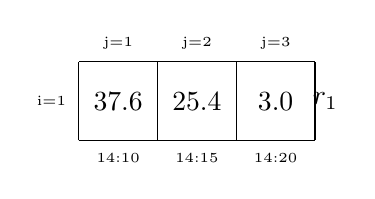
\begin{tikzpicture}
	\definecolor{mycolor}{RGB}{224,224,224}
	\definecolor{mycolor2}{RGB}{192,192,192}
	\draw[step=1cm,color=black] (0,0) grid (3,1);
	\node at (0.5,+0.5) [label={[font=\tiny,label distance=0.3cm]above:$\text{j=1}$}, label={[font=\tiny,label distance=0.1cm]left:$\text{i=1}$}, label={[font=\tiny,label distance=0.3cm]below:$\text{14:10}$}]{37.6};
	\node at (1.5,+0.5) [label={[font=\tiny,label distance=0.3cm]above:$\text{j=2}$},label={[font=\tiny,label distance=0.3cm]below:$\text{14:15}$}]{25.4};
	\node at (2.5,+0.5) [label=right:$r_1$,label={[font=\tiny,label distance=0.3cm]above:$\text{j=3}$},label={[font=\tiny,label distance=0.3cm]below:$\text{14:20}$}]{3.0};	
	\end{tikzpicture}
	\caption{Query Pattern $Q(\bar{t})$ of length $l=3$ and $d=1$ reference time series.}
	\label{Qpatt}
\end{figure}

\begin{figure}[H]
	\centering
	\begin{tikzpicture}[
	scale=0.7,
	every node/.style={outer sep=0pt, transform shape, font=\scriptsize},
	every matrix/.style={cells={scale=0.7}},
	]
	
		\definecolor{myorange}{RGB}{255,178,102}
		\definecolor{myblue}{RGB}{153,204,255}
		\definecolor{myyellow}{RGB}{255,255,102}
		
		% circular array
		\xyshift{-15mm}{-100mm}{
			\matrix [ampersand replacement=\&, outer sep=0pt, matrix anchor=north] (array) {
				\node[circularptr, fill=myblue] (c1)  {37.6}; \&
				\node[circularptr, fill=myorange] (c2)  {25.4}; \&
				\node[circularptr, fill=myyellow] (c3)  {3.0}; \&
				\node[circularptr] (c4)  {13.2}; \&
				\node[circularptr] (c5)  {23.0}; \&
				\node[circularptr] (c6)  {17.1}; \&
				\node[circularptr] (c7)  {37.6}; \&
				\node[circularptr] (c8)  {18.1}; \&
				\node[circularptr] (c9)  {7.2}; \&
				\node[circularptr] (c10) {25.4}; \&
				\node[circularptr] (c11) {38.9}; \&
				\node[circularptr] (c12) {47.1}; \&
				\node[circularptr] (c13) {43.1}; \&
				\node[circularptr] (c14) {2.5};  \\
				%
				\node[circularval, fill=myblue] (left) {14:10}; \&
				\node[circularval, fill=myorange] {14:15}; \&
				\node[circularval, fill=myyellow] {14:20}; \&
				\node[circularval] {13:15}; \&
				\node[circularval] {13:20}; \&
				\node[circularval] {13:25}; \&
				\node[circularval] {13:30}; \&
				\node[circularval] {13:35}; \&
				\node[circularval] {13:40}; \&
				\node[circularval] {13:45}; \&
				\node[circularval] {13:50}; \&
				\node[circularval] {13:55}; \&
				\node[circularval] {14:00}; \&
				\node[circularval] (right){14:05};\\
			};
		}
	

	
	
	
	% root node
	\xyshift{-20mm}{0mm}{\btreeinodethree{root}{17.1}{}{}};
	
	%
	% intermediate nodes
	\xyshift{-50mm}{-15mm}{\btreeinodethree{n1}{7.2}{}{}{}}
	\xyshift{ 10mm}{-15mm}{\btreeinodethree{n2}{23.0}{37.6}{43.1}}
	%
	% connecting root to intermediate level nodes
	\foreach \x in {1,2} { \btreelink{root-\x}{n\x} }
	%
	% leaf nodes
	\xyshift{-90mm}{-30mm}{\btreelnodethree{n11}{2.5}{3.0}{}}
	\xyshift{-60mm}{-30mm}{\btreelnodethree{n12}{7.2}{13.2}{}}
	\xyshift{-30mm}{-30mm}{\btreelnodethree{n21}{17.1}{18.1}{}}
	\xyshift{ 0mm}{-30mm}{\btreelnodethree{n22}{23.0}{25.4}{}}
	\xyshift{ 30mm}{-30mm}{\btreelnodethree{n23}{37.6}{38.9}{}}
	\xyshift{ 60mm}{-30mm}{\btreelnodethree{n24}{43.1}{47.1}{}}
	%
	% connecting intermediate level to leaf nodes
	\foreach \x in {1,2}     { \btreelink{n1-\x}{n1\x} }
	\foreach \x in {1,2,3,4} { \btreelink{n2-\x}{n2\x} }
	%
	% leaf pointers
	\draw[btlink] ([yshift=+3pt] n11-c.east) -- ([yshift=+3pt] n12-a.west);
	\draw[btlink] ([yshift=-3pt] n12-a.west) -- ([yshift=-3pt] n11-c.east);
	\draw[btlink] ([yshift=+3pt] n12-c.east) -- ([yshift=+3pt] n21-a.west);
	\draw[btlink] ([yshift=-3pt] n21-a.west) -- ([yshift=-3pt] n12-c.east);
	\draw[btlink] ([yshift=+3pt] n21-c.east) -- ([yshift=+3pt] n22-a.west);
	\draw[btlink] ([yshift=-3pt] n22-a.west) -- ([yshift=-3pt] n21-c.east);
	\draw[btlink] ([yshift=+3pt] n22-c.east) -- ([yshift=+3pt] n23-a.west);
	\draw[btlink] ([yshift=-3pt] n23-a.west) -- ([yshift=-3pt] n22-c.east);
	\draw[btlink] ([yshift=+3pt] n23-c.east) -- ([yshift=+3pt] n24-a.west);
	\draw[btlink] ([yshift=-3pt] n24-a.west) -- ([yshift=-3pt] n23-c.east);
	%
	
	% circular array
	\xyshift{-40mm}{-60mm}{
		\matrix [ampersand replacement=\&, outer sep=0pt, matrix anchor=north] (array) {
			\node[circularptr] (c1)  {}; \\	
			%
			\node[circularval] (left)(right) {13:45}; \\
		};
	}
	% circular array
	\xyshift{-10mm}{-60mm}{
		\matrix [ampersand replacement=\&, outer sep=0pt, matrix anchor=north] (array) {
		
			\node[circularptr, fill=myorange] (c2)  {}; \\	
			%	
				\draw node [black,midway,yshift=-1.3cm] {leftPos$^-$ = rightPos$^+$};
								\draw node [black,midway,yshift=-1.6cm] {$q_{1,2}$};
			\node[circularval,fill=myorange] (left)(right) {14:15}; \\
		};
	}	
	
	
		% circular array
		\xyshift{20mm}{-60mm}{
			\matrix [ampersand replacement=\&, outer sep=0pt, matrix anchor=north] (array) {
				\node[circularptr] (c5)  {}; \\	
				%
				\node[circularval] (left)(right) {13:30}; \\
			};
		}
		% circular array
		\xyshift{50mm}{-60mm}{
			\matrix [ampersand replacement=\&, outer sep=0pt, matrix anchor=north] (array) {
				\node[circularptr, fill=myblue] (c6)  {}; \\	
				%
				\draw node [black,midway,yshift=-1.3cm] {leftPos$^-$ = rightPos$^+$};
					\draw node [black,midway,yshift=-1.6cm] {$q_{1,1}$};
				\node[circularval,fill=myblue] (left)(right) {14:10}; \\
			};
		}	
		% draw pointers between circular array and B+ tree
		\path[btlink2] ([yshift=-2pt] c5.center)  edge[out=90,in=270] ([yshift=2pt] n23-1.center);
		% draw pointers for linked list
		\draw[btlink] ([yshift=-10pt] c5.east) -- ([yshift=-10pt] c6.west);
		\draw[btlink] ([yshift=-20pt] c6.west) -- ([yshift=-20pt] c5.east);
		
		%circular links
		\path[btlink] ([yshift=-10pt] c5.west)  edge[out=220,in=250] ([yshift=-10pt] c6.east);
		\path[btlink2] ([yshift=-20pt] c5.west)  edge[out=220,in=250] ([yshift=-20pt] c6.east);	
		
		
	
	% draw pointers between circular array and B+ tree
	\path[btlink2] ([yshift=-2pt] c1.center)  edge[out=90,in=270] ([yshift=2pt] n22-2.center);
	% draw pointers for linked list
	\draw[btlink] ([yshift=-10pt] c1.east) -- ([yshift=-10pt] c2.west);
	%\draw[btlink] ([yshift=-10pt] c2.east) -- ([yshift=-10pt] c1.east);
	\draw[btlink] ([yshift=-20pt] c2.west) -- ([yshift=-20pt] c1.east);
	
	%circular links
	\path[btlink] ([yshift=-10pt] c1.west)  edge[out=220,in=250] ([yshift=-10pt] c2.east);
	\path[btlink2] ([yshift=-20pt] c1.west)  edge[out=220,in=250] ([yshift=-20pt] c2.east);
	
	
	% list  value
	\xyshift{-90mm}{-50mm}{
		\matrix [ampersand replacement=\&, outer sep=0pt, matrix anchor=north] (array) {
			\node[circularptr] (c3)  {}; \\	
			%
			\node[circularval] (left)(right) {14:05}; \\
		};
	}
	
	% draw pointers between list value and B+ tree
	\path[btlink2] ([yshift=-2pt] c3.center)  edge[out=90,in=270] ([yshift=2pt] n11-1.center);
	
	%circular links
	\path[btlink] ([yshift=-16pt] c3.west)  edge[out=-1500,in=-60] ([yshift=-16pt] c3.east);
	\path[btlink2] ([yshift=-24pt] c3.west)  edge[out=-1500,in=-60] ([yshift=-24pt] c3.east);
	
	
	% list  value
	\xyshift{-70mm}{-50mm}{
		\matrix [ampersand replacement=\&, outer sep=0pt, matrix anchor=north] (array) {
			\node[circularptr,fill=myyellow] (c4)  {}; \\	
			%
			\draw node [black,midway,yshift=-0.9cm] {leftPos$^-$ = rightPos$^+$};
				\draw node [black,midway,yshift=-1.3cm] {$q_{1,3}$};
			\node[circularval, fill=myyellow] (left)(right) {14:20}; \\
		};
	}
	
	% draw pointers between list value and B+ tree
	\path[btlink2] ([yshift=-2pt] c4.center)  edge[out=90,in=270] ([yshift=2pt] n11-2.center);
	
	%circular links
	\path[btlink] ([yshift=-16pt] c4.west)  edge[out=-1500,in=-60] ([yshift=-16pt] c4.east);
	\path[btlink2] ([yshift=-24pt] c4.west)  edge[out=-1500,in=-60] ([yshift=-24pt] c4.east);
	
	\foreach \x in
	{n12-1,n12-2,n21-1,n21-2,n22-1, n23-2, n23-3, n24-1,n24-2}
	{ \path[<-] ([yshift=-15pt] \x.center) edge ([yshift=2pt] \x.center); }
	%
	

	\end{tikzpicture}
	\vspace{2mm}
	\caption{The circular array and the $B^+$tree for time series $r_1$ after initialization.}
	\label{fig:initialize}
\end{figure}

\begin{example}
	If $d=1$ just one time series included in query pattern $Q(\bar{t})$. Figure \ref{Qpatt} illustrates an example of a query pattern with $d=1$. In total $l$ neighborhoods are initialized for time series $r_1$. Figure \ref{fig:initialize} shows the circular array and the $B^+$tree for time series $r_1$ after the initialization. The coloured linked list elements represent the $leftPos^-$ and $rightPos^+$ of the newly initialized neighborhoods. 
\end{example}


\begin{algorithm}[H]
	\IncMargin{1em}
	\SetAlgoLined
	\DontPrintSemicolon
	\KwIn{Tree $tree$, the query pattern value $q_{i,j}$ and its time point $t$ and position $j$ and the pattern length $l$}
	\KwOut{The initialized neighborhood $N(q_{i,j})$}
	
	N.key $\leftarrow$ $q_{i,j}$\;
	N.j $\leftarrow$ $j$\;
	N.l $\leftarrow$ $l$\;
	
	\BlankLine
	leaf $\leftarrow$ FindLeaf(tree, $q_{i,j}$)\;
	i $\leftarrow$ smallest number such that $q_{i,j}$ $\leq$ leaf.$K_i$\;
	e $\leftarrow$ leaf.pointers[i]\;
	\BlankLine
	//Upper Bound: The value is at most pattern length away form first list value\;
	maxSteps $\leftarrow$ $l$\;
	\While{e.time $\neq$ t {\bf and} maxSteps $\neq$ 0}{
		//go from newest value back towards oldest\;
		e $\leftarrow$ e.prev\;
		maxSteps$--$\;
	}
	
	N.leftPos $\leftarrow$ set position to e\;
	N.rightPos $\leftarrow$ set position to e\;

	\Return N($q_{i,j}$);
	
	
	
	
	\caption{NewNeighborhood$(tree,q_{i,j},t,j,l)$}	\label{initializeNeighborhood}
\end{algorithm}




\subsection{Sorted Access}
After the initialization of the $l \times d$ neighborhoods the $k$ most non-overlapping patterns are calculated. Thus, the sortedAccess$(N(q_{i,j}),T)$ operation is executed until the $k$ patterns are retrieved. 
Sorted access searches the time point for the next most similar value to a query pattern cell $q_{i,j}$ of query pattern $Q(\bar{t})$. The Algorithm \ref{NeighborhoodGrow} presents the sorted access method. The neighborhood $N(q_{i,j})$ is expanded until such a value is retrieved. Some time points may have to be skipped because the time point anchored a pattern already and therefore not need to be considered again. The next unseen most similar value to $q_{i,j}$ is either at position $t^-$ or $t^+$, which represent the time points to the direct left or right of $leftPos^-$ and $rightPos^+$, respectively. If $|s_i(t^-) - q_{i,j}| \leq |s_i(t^+) - q_{i,j}|$ $leftPos^-$ is decremented to $prev(leftPos^-$) and $t=t^-$. $prev(leftPos^-)$ searches for the next previous measurement time point ($next(rightPos^-)$ vice versa). If $leftPos^-$ has a predecessor in the linked list of a leaf value $v$, which is not the tail, $prev(leftPos^-)$ is set to the predecessor, thus $prev(leftPos^-)$ is still in the same linked list. If there is no appropriate predecessor in the linked list, $prev(leftPos^-)$ is placed to the tail of the linked list associated to the leaf value on the left side next to $v$. If there is no value to the left side in the same leaf, the rightmost value in the left leaf sibling is used.

\begin{algorithm}[H]
	\IncMargin{1em}
	\SetAlgoLined
	\DontPrintSemicolon
	\KwIn{The neighborhood $N$ around query pattern value $q_{i,j}$ and the set of visited time points $T$}
	\KwOut{Time point of the next most similar value to $q_{i,j}$}
	
	
	leftPos$^-$ $\leftarrow$ N.leftPos\;
	rightPos$^+$ $\leftarrow$ N.rightPos\;
	
	
	\While{$t^-$ $\neq$ NIL {\bf and} ($t^-$ $-j + l$) $\in T$}{
		
		leftPos$^-$ $\leftarrow$ prev(leftPos$^-$)\;	}
	
	\While{$t^+$ $\neq$ NIL {\bf and}  ($t^+$ $-j + l$) $\in T$}{
		
		rightPos$^+$ $\leftarrow$ next(rightPos$^+$)\;
	}
	
	\uIf{$t^-$ $\neq$ NIL {\bf and}  $t^+$ $\neq$ NIL }{
		\eIf{$|r_{i}(t^-)$ - $q_{i,j}$$|$ $\leq$ $|r_{i}(t^+)$ - $q_{i,j}$$|$}{
			
			leftPos$^-\leftarrow$ prev(leftPos$^-$); $t$ $\leftarrow$ $t^-$\;
			
		}
		{
			rightPos$^+\leftarrow$ next(rightPos$^+$); $t$ $\leftarrow$ $t^+$\;
		}
	}
	\uElseIf{$t^-$ $\neq$ NIL}{
		
		leftPos$^-\leftarrow$ prev(leftPos$^-$); $t$ $\leftarrow$ $t^-$\;
	}
	\uElseIf{$t^+$ $\neq$ NIL}{
		rightPos$^+\leftarrow$ next(rightPos$^+$); $t$ $\leftarrow$ $t^+$\;
		
	}
	\Else{
		\Return NIL\; 	
	}
	
	
	\Return t\;
	
	
	
	
	\caption{SortedAccess$(N(q_{i,j}), T)$}	\label{NeighborhoodGrow}
\end{algorithm}

\begin{figure}[H]
	\centering
	\begin{tikzpicture}[
	scale=0.7,
	every node/.style={outer sep=0pt, transform shape, font=\scriptsize},
	every matrix/.style={cells={scale=0.7}},
	]
	
	\definecolor{myorange}{RGB}{255,178,102}
	\definecolor{myblue}{RGB}{51,153,255}
	\definecolor{myyellow}{RGB}{255,255,102}

	% leaf nodes
	\xyshift{-90mm}{-30mm}{\btreelnodethree{n11}{2.5}{3.0}{}}
	\xyshift{-60mm}{-30mm}{\btreelnodethree{n12}{7.2}{13.2}{}}
	\xyshift{-30mm}{-30mm}{\btreelnodethree{n21}{17.1}{18.1}{}}
	\xyshift{ 0mm}{-30mm}{\btreelnodethree{n22}{23.0}{25.4}{}}
	\xyshift{ 30mm}{-30mm}{\btreelnodethree{n23}{37.6}{38.9}{}}
	\xyshift{ 60mm}{-30mm}{\btreelnodethree{n24}{43.1}{47.1}{}}
	%
	% leaf pointers
	\draw[btlink] ([yshift=+3pt] n11-c.east) -- ([yshift=+3pt] n12-a.west);
	\draw[btlink] ([yshift=-3pt] n12-a.west) -- ([yshift=-3pt] n11-c.east);
	\draw[btlink] ([yshift=+3pt] n12-c.east) -- ([yshift=+3pt] n21-a.west);
	\draw[btlink] ([yshift=-3pt] n21-a.west) -- ([yshift=-3pt] n12-c.east);
	\draw[btlink] ([yshift=+3pt] n21-c.east) -- ([yshift=+3pt] n22-a.west);
	\draw[btlink] ([yshift=-3pt] n22-a.west) -- ([yshift=-3pt] n21-c.east);
	\draw[btlink] ([yshift=+3pt] n22-c.east) -- ([yshift=+3pt] n23-a.west);
	\draw[btlink] ([yshift=-3pt] n23-a.west) -- ([yshift=-3pt] n22-c.east);
	\draw[btlink] ([yshift=+3pt] n23-c.east) -- ([yshift=+3pt] n24-a.west);
	\draw[btlink] ([yshift=-3pt] n24-a.west) -- ([yshift=-3pt] n23-c.east);
	%
	
	% circular array
	\xyshift{-40mm}{-60mm}{
		\matrix [ampersand replacement=\&, outer sep=0pt, matrix anchor=north] (array) {
			\node[circularptr] (c1)  {}; \\	
			%
			\node[circularval] (left)(right) {13:45}; \\
		};
	}
	% circular array
	\xyshift{-10mm}{-60mm}{
		\matrix [ampersand replacement=\&, outer sep=0pt, matrix anchor=north] (array) {
			\node[circularptr, fill=myorange] (c2)  {}; \\	
			%
			\draw node [black,midway,yshift=-1.3cm] {leftPos$^-$ = rightPos$^+$};
			\node[circularval,fill=myorange] (left)(right) {14:15}; \\
		};
	}	
	
	
	% circular array
	\xyshift{20mm}{-60mm}{
		\matrix [ampersand replacement=\&, outer sep=0pt, matrix anchor=north] (array) {
			\node[circularptr] (c5)  {}; \\	
			%
			\node[circularval] (left)(right) {13:30}; \\
		};
	}
	% circular array
	\xyshift{50mm}{-60mm}{
		\matrix [ampersand replacement=\&, outer sep=0pt, matrix anchor=north] (array) {
			\node[circularptr] (c6)  {}; \\	
			%
			\node[circularval] (left)(right) {14:10}; \\
		};
	}	
	% draw pointers between circular array and B+ tree
	\path[btlink2] ([yshift=-2pt] c5.center)  edge[out=90,in=270] ([yshift=2pt] n23-1.center);
	% draw pointers for linked list
	\draw[btlink] ([yshift=-10pt] c5.east) -- ([yshift=-10pt] c6.west);
	\draw[btlink] ([yshift=-20pt] c6.west) -- ([yshift=-20pt] c5.east);
	
	%circular links
	\path[btlink] ([yshift=-10pt] c5.west)  edge[out=220,in=250] ([yshift=-10pt] c6.east);
	\path[btlink2] ([yshift=-20pt] c5.west)  edge[out=220,in=250] ([yshift=-20pt] c6.east);	
	
	
	
	% draw pointers between circular array and B+ tree
	\path[btlink2] ([yshift=-2pt] c1.center)  edge[out=90,in=270] ([yshift=2pt] n22-2.center);
	% draw pointers for linked list
	\draw[btlink] ([yshift=-10pt] c1.east) -- ([yshift=-10pt] c2.west);
	%\draw[btlink] ([yshift=-10pt] c2.east) -- ([yshift=-10pt] c1.east);
	\draw[btlink] ([yshift=-20pt] c2.west) -- ([yshift=-20pt] c1.east);
	
	%circular links
	\path[btlink] ([yshift=-10pt] c1.west)  edge[out=220,in=250] ([yshift=-10pt] c2.east);
	\path[btlink2] ([yshift=-20pt] c1.west)  edge[out=220,in=250] ([yshift=-20pt] c2.east);


	

	
	\foreach \x in
	{n11-1,n11-2,n12-1,n12-2,n21-1,n21-2,n22-1, n23-2, n23-3, n24-1,n24-2}
	{ \path[<-] ([yshift=-15pt] \x.center) edge ([yshift=2pt] \x.center); }
	%
	
	
	%second
	
	
	
		% leaf nodes
		\xyshift{-90mm}{-90mm}{\btreelnodethree{xn11}{2.5}{3.0}{}}
		\xyshift{-60mm}{-90mm}{\btreelnodethree{xn12}{7.2}{13.2}{}}
		\xyshift{-30mm}{-90mm}{\btreelnodethree{xn21}{17.1}{18.1}{}}
		\xyshift{ 0mm}{-90mm}{\btreelnodethree{xn22}{23.0}{25.4}{}}
		\xyshift{ 30mm}{-90mm}{\btreelnodethree{xn23}{37.6}{38.9}{}}
		\xyshift{ 60mm}{-90mm}{\btreelnodethree{xn24}{43.1}{47.1}{}}
		%
		% leaf pointers
		\draw[btlink] ([yshift=+3pt] xn11-c.east) -- ([yshift=+3pt] xn12-a.west);
		\draw[btlink] ([yshift=-3pt] xn12-a.west) -- ([yshift=-3pt] xn11-c.east);
		\draw[btlink] ([yshift=+3pt] xn12-c.east) -- ([yshift=+3pt] xn21-a.west);
		\draw[btlink] ([yshift=-3pt] xn21-a.west) -- ([yshift=-3pt] xn12-c.east);
		\draw[btlink] ([yshift=+3pt] xn21-c.east) -- ([yshift=+3pt] xn22-a.west);
		\draw[btlink] ([yshift=-3pt] xn22-a.west) -- ([yshift=-3pt] xn21-c.east);
		\draw[btlink] ([yshift=+3pt] xn22-c.east) -- ([yshift=+3pt] xn23-a.west);
		\draw[btlink] ([yshift=-3pt] xn23-a.west) -- ([yshift=-3pt] xn22-c.east);
		\draw[btlink] ([yshift=+3pt]xn23-c.east) -- ([yshift=+3pt] xn24-a.west);
		\draw[btlink] ([yshift=-3pt] xn24-a.west) -- ([yshift=-3pt] xn23-c.east);
		%
		
		% circular array
		\xyshift{-40mm}{-120mm}{
			\matrix [ampersand replacement=\&, outer sep=0pt, matrix anchor=north] (array) {
				\node[circularptr,fill=myorange] (xc1)  {}; \\	
				%

				\node[circularval,fill=myorange] (left)(right) {13:45}; \\
			};
		}
		% circular array
		\xyshift{-10mm}{-120mm}{
			\matrix [ampersand replacement=\&, outer sep=0pt, matrix anchor=north] (array) {
				\node[circularptr, fill=myorange] (xc2)  {}; \\	
				%
			\draw node [black,midway,yshift=-1.1cm] {rightPos$^+$};
				\node[circularval,fill=myorange] (left)(right) {14:15}; \\
			};
		}	
		
		
		% circular array
		\xyshift{20mm}{-120mm}{
			\matrix [ampersand replacement=\&, outer sep=0pt, matrix anchor=north] (array) {
				\node[circularptr] (xc5)  {}; \\	
				%
				\node[circularval] (left)(right) {13:30}; \\
			};
		}
		% circular array
		\xyshift{50mm}{-120mm}{
			\matrix [ampersand replacement=\&, outer sep=0pt, matrix anchor=north] (array) {
				\node[circularptr] (xc6)  {}; \\	
				%
				\node[circularval] (left)(right) {14:10}; \\
			};
		}	
		% draw pointers between circular array and B+ tree
		\path[btlink2] ([yshift=-2pt] xc5.center)  edge[out=90,in=270] ([yshift=2pt] xn23-1.center);
		% draw pointers for linked list
		\draw[btlink] ([yshift=-10pt] xc5.east) -- ([yshift=-10pt] xc6.west);
		\draw[btlink] ([yshift=-20pt] xc6.west) -- ([yshift=-20pt] xc5.east);
		
		%circular links
		\path[btlink] ([yshift=-10pt] xc5.west)  edge[out=220,in=250] ([yshift=-10pt] xc6.east);
		\path[btlink2] ([yshift=-20pt] xc5.west)  edge[out=220,in=250] ([yshift=-20pt] xc6.east);	
		
		
		
		% draw pointers between circular array and B+ tree
		\path[btlink2] ([yshift=-2pt] xc1.center)  edge[out=90,in=270] ([yshift=2pt] xn22-2.center);
		% draw pointers for linked list
		\draw[btlink] ([yshift=-10pt] xc1.east) -- ([yshift=-10pt] xc2.west);
		%\draw[btlink] ([yshift=-10pt] c2.east) -- ([yshift=-10pt] c1.east);
		\draw[btlink] ([yshift=-20pt] xc2.west) -- ([yshift=-20pt] xc1.east);
		
		%circular links
		\path[btlink] ([yshift=-10pt] xc1.west)  edge[out=220,in=250] ([yshift=-10pt] xc2.east);
		\path[btlink2] ([yshift=-20pt] xc1.west)  edge[out=220,in=250] ([yshift=-20pt] xc2.east);
		
		
			% list  value
			\xyshift{-60mm}{-120mm}{
				\matrix [ampersand replacement=\&, outer sep=0pt, matrix anchor=north] (array) {
					\node[circularptr,fill=myorange] (c3)  {}; \\	
					%
					\node[circularval,fill=myorange] (left)(right) {13:20}; \\
				};
			}
			
			% draw pointers between list value and B+ tree
			\path[btlink2] ([yshift=-2pt] c3.center)  edge[out=90,in=270] ([yshift=2pt] xn22-1.center);
			
			%circular links
			\path[btlink] ([yshift=-16pt] c3.west)  edge[out=-1500,in=-60] ([yshift=-16pt] c3.east);
			\path[btlink2] ([yshift=-24pt] c3.west)  edge[out=-1500,in=-60] ([yshift=-24pt] c3.east);
		
				
				% list  value
				\xyshift{-80mm}{-120mm}{
					\matrix [ampersand replacement=\&, outer sep=0pt, matrix anchor=north] (array) {
						\node[circularptr,fill=myorange] (c7)  {}; \\	
						%
						\draw node [black,midway,yshift=-1.1cm] {leftPos$^-$};
						\node[circularval,fill=myorange] (left)(right) {13:35}; \\
					};
				}
				
				% draw pointers between list value and B+ tree
				\path[btlink2] ([yshift=-2pt] c7.center)  edge[out=90,in=270] ([yshift=2pt] xn21-2.center);
				
				%circular links
				\path[btlink] ([yshift=-16pt] c7.west)  edge[out=-1500,in=-60] ([yshift=-16pt] c7.east);
				\path[btlink2] ([yshift=-24pt] c7.west)  edge[out=-1500,in=-60] ([yshift=-24pt] c7.east);
				
		
		
		\foreach \x in
		{xn11-1,xn11-2,xn12-1,xn12-2,xn21-1, xn23-2, xn23-3, xn24-1,xn24-2}
		{ \path[<-] ([yshift=-15pt] \x.center) edge ([yshift=2pt] \x.center); }
		%
		
		
	
	
	
	\end{tikzpicture}
	\vspace{2mm}
	\caption{Status of $N(q_{1,2})$ after growing 3 times.}
	\label{fig:increase}
\end{figure}

\begin{example}
	Figure \ref{fig:increase} shows how the neighborhood $N(q_{1,2})$ is expanded. We assume that the other neighborhoods $N(q_{1,1})$ and $N(q_{1,3})$ have not been initialized yet. 
	Hence, there are no additional time points anchored for a pattern previously and the timeset $T$ is initially empty. If the sortedAccess$(N(q_{i,j}),T)$ is executed 3 times the resulting neighborhood is illustrated in Figure \ref{fig:increase}.
\end{example}



\chapter{Complexity Analysis}
\label{Complexity}
This analysis refers to a single time series $s$ for which a $B^+$tree and a circular array are maintained and the complexity calculations are valid for our context, e.g. the linked list elements are traversed at most $l$ times. 
\newtheorem{mydef}{Lemma}

\section{Runtime Complexity}

\paragraph{Circular, Doubly Linked List}
\begin{mydef}
	The insertion of a new time point to a linked list needs $O(1)$ time.
	\label{circ:def1}
\end{mydef}
\begin{proof}
	For each new value produced by a time series $s$ a linked list in the $B^+$tree is expanded. Since the new value is always inserted at the tail position it needs $O(1)$ time.
\end{proof}
\begin{mydef}
	The deletion of a time point from a linked list needs $O(1)$ time.
	\label{circ:def2}
\end{mydef}
\begin{proof}
	For each deletion in a $B^+$tree a time point needs to be removed from a linked list. Since the oldest value is always at the head position, the deletion needs $O(1)$ time.
\end{proof}


\paragraph{Circular Array Operations}
\begin{mydef}
	The update of the circular array takes $O(1)$ time.
	\label{updateAC}
\end{mydef}
\begin{proof}
	The next update position in a circular array is computed in $O(1)$ time, hence the update takes $O(1)$ time. 
\end{proof}
\begin{mydef}
	The random access of a time point $t$ takes $O(1)$ time.
\end{mydef}
\begin{proof}
	The random access algorithm needs to calculate the position for the time point $t$. Since the position can be calculated using the $lastPos$ and the time interval, it takes $O(1)$ time.
\end{proof}

\subsubsection{$B^+$tree Operations}

Normally, the complexity of $B^+$tree operations is dependent on the 
required disk I/O operations because I/O operations are expensive. The speed of operations on $B^+$trees makes it a frequently used index structure in database implementations. But we do not have disk I/O operations, hence, the complexity of our implementation also depends on the tree node size which usually is neglected because it is not as expensive as disk I/O operations. 
\\Since we have no disk I/O operation the parameter $n$ has an influence on our complexity. For every node visited we pay $O(n)$ time to find the position of a value. The parameter $|W|$ has an influence as well since 
there are at most $|W|$ keys in $B^+$tree leaves (provided that there are no duplicate values).

\begin{mydef}
	Finding a leaf in the $B^+$tree takes at most $O(n \times \log_{n}|W|)$ time.
	\label{def:find}
\end{mydef}
\begin{proof}
 The nodes are traversed recursively downwards from the root of the tree to its leaves.  In the worst case, the number of nodes that must be traversed is $log_{n}|W|$. This leads to $log_{n}|W|$ complexity, where $|W|$ is the maximum total number of keys in the leaves and $n$ is representing the maximum number of pointers in an inner node. \\Additionally, you pay for every node that is visited $O(n)$ time to find the index position to the child node. Hence, the total complexity to find a leaf takes $O(n \times \log_{n}|W|)$ time. 
\end{proof}



\begin{mydef}
	The insertion of a measurement to the $B^+$tree takes $O(n \times \log_{n}(|W|))$ time.
\end{mydef}
\begin{proof}
	Before a measurement can be inserted to the tree the appropriate leaf has to be found. Lemma \ref{def:find} states that this takes $O(n \times \log_{n}(|W|))$ time.
	The addition of a measurement can cause three different cases as explained in Section \ref{insertionTree}. 
	\begin{itemize}
		\item (The key already exists) Lemma \ref{circ:def1} states that a measurement can be inserted in $O(1)$ time to the linked list. 
		\item (The node has still room and the measurement is inserted to the node)
		This causes that the insertion place has to be found which takes at most $O(n)$ time, since the keys have to remain ordered. 
		\item (The node is already full and the node has to split) To split the node it takes $O(n)$ time. Because the keys have to remain ordered, the insertion point is found by traversing the keys. After the keys are distributed to both nodes in $O(n)$ time. If the tree is recursively traversed upwards, at most $\log_{n}|W|$ nodes are split which results in a total time complexity of $n \times \log_{n}|W|$.
	\end{itemize}
	Since the time complexity to find a leaf is $O(n \times \log_{n}|W|)$ which is equal to the time complexity of a redistribution, the overall time complexity of an insertion is $O(n \times \log_{n}|W|)$.
\end{proof}


\begin{mydef}
	The deletion of a measurement from the $B^+$tree takes $O(n \times \log_{n}|W|)$ time.
\end{mydef}
\begin{proof}
	Before a measurement is deleted from the tree the appropriate leaf has to be found. Lemma \ref{def:find} states that this takes $O(n \times \log_{n}|W|)$ time.
	The deletion of a measurement can cause four different cases as explained in Section \ref{deleteTree}. 
	\begin{itemize}
		\item (The measurement time point is a linked list element which contains multiple elements) Lemma \ref{circ:def2} states that a measurement can be deleted in $O(1)$ time from the linked list. Hence, duplicates have no influence on the complexity of a deletion. 
		\item (The node is at least half-full) If the node has still enough keys the entry is searched in $O(n)$ time by traversing the node keys and then is deleted. 
		\item (The values in a node are redistributed) The redistribution is done by moving keys and pointers. At most $n$ keys have to be shifted which cost $O(n)$ time.
		\item (The node is merged with a sibling) To merge two nodes the keys and pointers have to be moved which costs at most $O(n)$ time. If the nodes are traversed upwards, there are at most $O(\log_{n}|W|)$ nodes to merge. Hence, the time complexity of the merge is $O(n \times \log_{n}|W|)$.
	\end{itemize}
	Since the time complexity to find a leaf is $O(n \times \log_{n}|W|)$ is equal to the time complexity of merge, the overall runtime complexity of deletion is $O(n \times \log_{n}|W|)$.
\end{proof}



\begin{mydef}
	The shift$(tree, array, \bar{t}, v)$ takes $O(n \times \log_{n}|W|)$ time.
	\label{shiftC}
\end{mydef}
\begin{proof}
The total time complexity of a shift depends on the following operations:
	\begin{itemize}
		\item The update of the circular array takes $O(1)$ as stated in Lemma \ref{updateAC}.
		\item The deletion of a measurement to the $B^+$tree takes $O(n \times \log_{n}|W|)$ time.
		\item The insertion of a measurement to the $B^+$tree takes $O(n \times \log_{n}|W|)$ time.
	\end{itemize}
	$O(n \times \log_{n}|W|)$ dominates the overall time complexity, this leads to a time complexity of $O(n \times \log_{n}|W|)$ for the shift operation. 
\end{proof}



\subsubsection{Neighborhood Operations}
 The newNeighborhood$(tree,q_{i,j},t,j,l)$ operation searches a specific measurement. Therefore, it cannot just take the tail or head position in a linked list like the insertion or deletion method. We initialize $l$ $\times$ $d$ neighborhoods, one for each value in a query pattern $Q(\bar{t})$. Thus, $l$ neighborhoods in every time series $r$ which are part of the pattern. The \emph{newNeighborhood} method always is executed at the $l$ newest measurements in an involved time series because the query pattern is anchored at the newest time point $\bar{t}$. Thus, we can give an upper bound, namely the pattern length $l$. As a consequence, at most $l$ element examinations in a linked list are necessary, where $l$ represents the pattern length.
 
 \begin{mydef}
 	The search of a specific time point in a linked list for newNeighborhood$(q_{i,j},t,j,l)$ is executed takes at most $O(l)$ time.
 	\label{circ:def3}
 \end{mydef}
 \begin{proof}
 	A time series $s$ in a pattern $P(t)$ initializes $l$ neighborhoods. Hence, in the worst case the $l$ newest measurements in the circular array for $s$ have the same value and thus, are stored in the same linked list in the $B^+$tree. Therefore, $l$ list elements have to be traversed to find the specific measurement time point, starting from the tail and scanning backwards. 
 \end{proof}
 
\begin{mydef}
	The initialization of a neighborhood in time series $s$ takes $O(l+(n \times \log_{n}|W|))$ time. \label{initNC}
\end{mydef}
\begin{proof}
	The initialization of the neighborhood needs to search a specific measurement in the $B^+$tree. Hence the complexity to find the measurement leaf is equal to the find leaf operation defined in Lemma \ref{def:find}. At most $l$ linked list elements are traversed as stated in Lemma \ref{circ:def3}. This leads to a total complexity of $O(l+(n \times \log_{n}|W|))$.
\end{proof}

\begin{mydef}
	The sortedAccess$(N(q_{i,j}),T)$ takes at most $O(|T|)$ time. \label{sAC}
\end{mydef}
\begin{proof}
	If the timeset contains $|T|$ time points and since at most $|T|$ time points have to be skipped the sortedAccess$(N(q_{i,j}),T)$ takes at most at most $O(|T|)$ time. 
\end{proof}

\section{Space Complexity}

\begin{mydef}
	The space complexity of a circular array is $O(|W|)$.
\end{mydef}
\begin{proof}
	Every circular array for a time series $s$ has a size $|W|$. Hence, the space complexity of one circular array is $O(|W|)$.
\end{proof}


\begin{mydef}
	The space complexity of a $B^+$tree is $O(|W|)$. 
\end{mydef}
\begin{proof}
	Each measurement is stored once in the tree. In the worst case, all values are unique and $|W|$ values are stored in leaves which cause a space complexity of $O(|W|)$. The number of keys in inner nodes and the root is always smaller than the number of keys in the leaf level. Hence, the space complexity of the leaf level determines the overall space complexity.
\end{proof}

\chapter{Experimental Evaluation}
\label{sec:Experimental}
This Chapter describes our experimental setup, the experiments and their results. We evaluated the running time of the shift, the sorted access and the newNeighborhood operation with different parameters. We did not include random access, because its time complexity is constant.


\section{Setup}
\label{setup}
In the experiments we construct a data set with measurement values with a time span of $100$ years between the newest and the oldest value. We use one time series $r$, thus $d=1$. The interval between two values is set to $3$ minutes. Since 20 measurements arrive per hour the data set contains in total $17'520'000$ measurements in $100$ years. The window size $|W|$ is set to 3 years ($525'600$). The data set contains values randomly chosen between $0$ and $10'000$ and duplicates are possible.


\section{Runtime}

\subsection{Shift}

\subsubsection{Increased Tree Node Size}

\paragraph{Aim}

This experiment tries to illustrate the effect of an increased tree node size $n-1$ on the shift operation. Besides, it wants to show that using a $B^+$tree was an appropriate choice.

\paragraph{Method}
To evaluate the influence of the tree node size on the runtime of the shift operation we executed the shift with values of the dataset introduced in Section \ref{setup}. For each tree node size represented in Figure \ref{tab:1} we made $3 \times 1'000'000$ shifts to eliminate outliers.

\paragraph{Variables}
We measure the runtime of the algorithm with different tree node sizes $n-1$. Therefore, the window size $|W|$ remains fixed to 3 years. The experiment starts with a tree node size $n-1 = 1$.

\paragraph{Prediction}
We expect that the tree node size influences the runtime as we described in Lemma \ref{shiftC}, which is nearly linear. Besides, we expect that the graph shows a minimum at a tree node size slightly larger than $1$. Otherwise, e.g. a red-black tree might have been a better choice because red-black tree has a tree node size of $1$\cite{RedBlackTree}.

\paragraph{Results}
Figure \ref{tab:1} shows that the parameter $n$ indeed has an influence on the running time. We observe that the algorithm had the best running time with a tree node size around $11$. A bigger or smaller tree node size decelerate the runtime. After the minimum is achieved the runtime is nearly linear with an increasing tree node size.



\begin{figure}[H]
	\centering
	\begin{tikzpicture}
	\begin{axis}[ width=0.8\textwidth,
	height=0.5\textwidth,
	width=0.9\linewidth, % Scale the plot to \linewidth
	grid=major, % Display a grid
	grid style={dashed,gray!50}, % Set the style
	xlabel=node size $n-1$, % Set the labels
	ylabel=runtime $\lbrack s \rbrack$
	={at={(2,-5)},anchor=north}, % Put the legend below the plot
	x label style={at={(axis description cs:0.5,-0.03)},anchor=north},
	y label style={at={(axis description cs:-0.01,.5)},anchor=south},
	x tick label style={rotate=90,anchor=east} % Display labels sideways
	]
	\addplot 
	% add a plot from table; you select the columns by using the actual name in
	% the .csv file (on top)
	table[x=Nodesize,y=s,col sep=comma] {experimenttreeNodeSize.csv}; 
	\legend{Runtime}
	\end{axis}
	\end{tikzpicture}
	\caption{Shift operation with increasing values for $n-1$.} \label{tab:1}
\end{figure}

\subsubsection{Increased Window Size}

\paragraph{Aim}

This experiment attempts to illustrate the effect of an increased window size $|W|$ on the performance of the shift operation. 

\paragraph{Method}
To evaluate the influence of window size $|W|$, we executed the shift over a different dataset than in the first experiment. This dataset has the same size as the dataset described in Section \ref{setup} but contains values randomly chosen between $0$ and $100'000$, thus $10$ times more distinct values are possible. The dataset is modified because the insertion of a duplicate value does not enlarge the height of the $B^+$tree and therefore should have no effect on the runtime of the shift with an enlarged window size $|W|$. For each window size $|W|$ we made $3 \times 1'700'000$ shifts to keep the outliers as small as possible. 

\paragraph{Variables}
We measure the runtime of the algorithm with different window sizes $|W|$. Therefore, the tree node size remains fix and is set to $11$ because the runtime for this tree node size was the minimum in the experiment illustrated in Figure \ref{tab:1}.  

\paragraph{Prediction}
We expect that the window size influences the runtime as we described in Lemma \ref{shiftC}. But we except that the window size $|W|$ only influences the runtime until no additional distinct values arrive. Hence, we expect an increasing runtime until the window has a size of $100'000$. We predict that a larger window size also causes fewer deletes. The circular array only has cheap list operations instead of expensive structural changes like the $B^+$tree. This reduces the runtime for a larger window $|W|$ for the first updates which do not delete a measurement from the $B^+$tree. To reduce this effect we make $1'700'000$ shifts instead of $1'000'000$. 

\paragraph{Results}
Figure \ref{fig:window} shows that the parameter $|W|$ influences the runtime of a shift. As expected, the runtime increases until the window size has achieved a size around $|W| = 100'000$. Afterwards, it decreases slightly. This can be explained with the increased window size which results in fewer measurement deletions. Hence, a larger window size has two different effects on the runtime. On the one hand, it increases the height of the $B^+$tree which increases the runtime for $|W|$ up to $100'000$ and on the other hand, a larger window size for $|W|>100'000$ significances less deletions from the $B^+$tree which decreases the runtime.



\begin{figure}[H]
	\centering
\begin{tikzpicture}
\begin{axis}[ width=0.8\textwidth,
height=0.5\textwidth,
width=0.9\linewidth, % Scale the plot to \linewidth
grid=major, % Display a grid
grid style={dashed,gray!50}, % Set the style
xlabel=$|W|$, % Set the labels
ylabel=runtime $\lbrack s \rbrack$
={at={(2,-5)},anchor=north}, % Put the legend below the plot
x label style={at={(axis description cs:0.5,-0.03)},anchor=north},
y label style={at={(axis description cs:-0.01,.5)},anchor=south},
x tick label style={rotate=90,anchor=east} % Display labels sideways  
]
\addplot 
% add a plot from table; you select the columns by using the actual name in
% the .csv file (on top)
table[x=W,y=s,col sep=comma] {experimentwindowSize.csv}; 
\legend{Runtime}
\end{axis}
\end{tikzpicture}
	\caption{Shift operation with increasing values for $|W|$.} \label{fig:window}
\end{figure}


\subsection{New Neighborhood}


\paragraph{Aim}

This experiment attempts to show the effect of an increased pattern length $l$ on the new neighborhood operation. We try to show that the pattern length $l$ has a very small influence to the runtime, which would support the usage of linked lists. 

\paragraph{Method}
To evaluate the influence of the pattern length on the runtime of the new neighborhood operation, we executed the operation with values of a dataset with again $17'520'000$ values but only $1'000$ possible distinct values. This leads to many duplicate values.  The window size $|W|$ is set to $17'520'000$ as well, to enhance the effect of duplicate values.
We measure the runtime of the neighborhood initialization for a measurement at position $\bar{t}-l$ for different pattern lengths. The $B^+$ tree is shifted $1'000'000$ times and then the initialization is executed. 

\paragraph{Variables}
We set the tree node size to $11$ and the window size to $6$ years. This leads to more duplicate values which should increase the effect of $l$.  We have a maximum pattern length of $9'000$. 

\paragraph{Prediction}
We expect that the tree node size influences the runtime linearly as we described in Lemma \ref{initNC}. In our case, the influence is expected to be visible because the tree contains many duplicate values. The pattern length only has an influence if the value $q_{i,l}$ occurs multiple times in time window $W$.  

\paragraph{Results}
As expected, the pattern length in our experiment has a visible influence on the runtime because the dataset contains many duplicate values. An increased pattern length leads to a worse runtime. However, we have many duplicates in our example. Since the values in our dataset are randomly chosen between $0$ and $1'000$ there can be values that occur more often than others. This influences the runtime, since sometimes fewer linked list values have to be examined although $l$ is higher. 


\begin{figure}[H]
	\centering
	\begin{tikzpicture}
	\begin{axis}[ width=0.8\textwidth,
	height=0.5\textwidth,
	width=0.9\linewidth, % Scale the plot to \linewidth
	grid=major, % Display a grid
	grid style={dashed,gray!50}, % Set the style
	xlabel=$l$, % Set the labels
	ylabel=runtime $\lbrack ms \rbrack$ 
	={at={(2,-5)},anchor=north}, % Put the legend below the plot
	x label style={at={(axis description cs:0.5,-0.03)},anchor=north},
	y label style={at={(axis description cs:-0.01,.5)},anchor=south},
	x tick label style={rotate=90,anchor=east} % Display labels sideways
	]
	\addplot 
	% add a plot from table; you select the columns by using the actual name in
	% the .csv file (on top)
	table[x=l,y=ms,col sep=comma] {experimentOneNeighborhoodInit2.csv}; 
	\legend{Runtime}
	\end{axis}
	\end{tikzpicture}
	\caption{Initialize neighborhood for a measurement at pattern cell $q_{i,l}$ } \label{fig:l}
\end{figure}




\subsection{Sorted Access}

\paragraph{Aim}

This experiment attempts to illustrate the effect of timeset $T$ on the runtime of the sorted access method. 

\paragraph{Method}
To evaluate the influence of the timeset on the runtime of the sorted access operation, we execute the sorted access on a $B^+$tree filled with values of the dataset introduced in \ref{setup}. The window size $|W|$ is set to 3 years and the tree node size to $11$. The timeset is filled with time points that need to be skipped by the algorithm, hence $t^- -j +l\in T$. We have no time points $t^+ -j + l \in T$. The graph would show if there exists no more time points to the left side of $N(q_{i,j})$ and the condition would be renewed. At first, the timeset contains only five values that need to be skipped. After, every time $10$ more values are added. We increase the number of time points $t^- -j + l \in T$, such that the while loop is executed every time $|T|$ times. The test is executed 3 times and the average runtime is calculated. The timeset for every execution is renewed, such that time points $t \in T$ are never skipped because they have been seen before. Furthermore, before each execution the neighborhood is initialized again. 

\paragraph{Variables}
We measure the runtime of the sorted access algorithm with a fix tree node size and a fix window size $|W|$ but each time for a different timeset $|T|$. 

\paragraph{Prediction}
We expect that the timeset $T$ has a linear influence on the runtime as we described in Lemma \ref{sAC}, since for every skipped time point the sorted access is expected to be slower. Therefore, we expect a linear graph. 

\paragraph{Results}
Figure \ref{fig:sorted} illustrates the results. We can see that the graph is nearly linear, which was expected. Although, the graph is not exactly linear this could be due to outliers.

\begin{figure}[H]
	\centering
	\begin{tikzpicture}
	\begin{axis}[ width=0.8\textwidth,
	height=0.6\textwidth,
	width=0.9\linewidth, % Scale the plot to \linewidth
	grid=major, % Display a grid
	grid style={dashed,gray!50}, % Set the style
	xlabel=$|T|$, % Set the labels
	ylabel=runtime $\lbrack ms \rbrack$
	={at={(2,-5)},anchor=north}, % Put the legend below the plot
	x label style={at={(axis description cs:0.5,-0.03)},anchor=north},
	y label style={at={(axis description cs:-0.01,.5)},anchor=south},
	x tick label style={rotate=90,anchor=east} % Display labels sideways
	]
	\addplot 
	% add a plot from table; you select the columns by using the actual name in
	% the .csv file (on top)
	table[x=T,y=ms,col sep=comma] {experimentSortedAccess23.csv}; 
	\legend{Runtime}
	\end{axis}
	\end{tikzpicture}
	\caption{Grow neighborhood with an increasing timeset size $|T|$.} \label{fig:sorted}
\end{figure}

\chapter{Summary and Conclusion}
\label{sec:Summary}
We studied the requirements to keep a portion of a streaming time series in main memory and simultaneously provide efficient access possibilities to past time series data. The system we presented uses two different data structures to achieve efficient access: a $B^+$tree and a circular array. Random access is efficiently performed on a circular array and sorted access is efficiently performed on a $B^+$tree with leaves linked to the respective successor and predecessor. Furthermore, the thesis introduces a possibility to handle duplicate values in a $B^+$tree with a simple but powerful linked list. The duplicate handling is not only simple to implement but also effective in terms of update velocity. Moreover, in our context, retrieving a specific value in the linked list has an upper bound. We presented the algorithms to implement this system and analysed their runtime and space complexity. Finally, we evaluated the performance of the system to underpin our theoretical results.






\begin{thebibliography}{99}
	\bibliographystyle{alpha}
	
	\bibitem{BScT} K. Wellenzohn, M. Böhlen, A. Dignös, J. Gamper, and H. Mitterer: \emph{Continuous Imputation of Missing Values in Streams of Pattern-Determining Time Series}; Unpublished, 2016.
	
	\bibitem{DatabaseSystemC} Abraham Silberschatz, Henry F. Korth, S. Sudarshan: \emph{Database System Concepts}; The McGraw-Hill Companies, Inc., New York, USA, pages 485-500, 2011. 
	
	\bibitem{LinkedListBook} Thomas H. Cormen, Charles E. Leiserson, Ronald L.Rivest, Clifford Stein: \emph{Introduction to Algorithms}; Massachusetts Institute of Technology, Massachusetts, USA, pages 236-241, 2009. 
	
	\bibitem{RedBlackTree} Mark Allen Weiss: \emph{Data Structures \& Algorithm Analysis in Java}; Florida International University, Florida, USA, pages 460-468, 1999. 
	
	
\end{thebibliography}




\appendix%*{Appendix}

\appendixpage


\addappheadtotoc
\chapter{Algorithms}

\label{app:Algo}

\section{$B^+$tree Deletion}
\label{app:Del}

\begin{algorithm}[H]
	\IncMargin{1em}
	\SetAlgoLined
	\DontPrintSemicolon
	\KwIn{Tree $tree$}
	\KwOut{The $tree$ with an adjusted root node}
	
	//enough keys in the root\;
	\If{0 < tree.root.numOfKeys}{
		\Return\; 	
	}
	//if the root has a child, promote the first (only) child as the new root\;
	\eIf{root is not a leaf}{
		newRoot $\leftarrow$ tree.root.pointers[0]\;
		newRoot.parent $\leftarrow$ NIL\;
	}
	{
		newRoot $\leftarrow$ NIL\;
	}
	
	tree.root $\leftarrow$ newRoot\;
	
	\caption{AdjustRoot$(tree)$}	\label{adjustTheRoot}
\end{algorithm}

\begin{algorithm}[H]
	\IncMargin{1em}
	\SetAlgoLined
	\DontPrintSemicolon
	\KwIn{Tree $tree$, the $node$ and its neighbor $neighbor$, the neighborIndex $nIndex$ and the key $kPrime$}
	\KwOut{$node$ and its $neighbor$ are merged to one node}
	
	//Swap neighbor with node if node is on the extreme left and neighbor is to its right\;
	\If{nIndex = -1}{
		swap neighbor with node\;
	}
	neighborInsertionIndex $\leftarrow$ neighbor.numOfKeys\;
	
	\eIf{node is no leaf}{
		neighbor.keys[neighborInsertionIndex] $\leftarrow$ kPrime\;
		neighbor.numOfKeys++\;
		decreasingIndex $\leftarrow$ 0\;
		numOfKeysBefore $\leftarrow$ node.numOfKeys\;
		\For{i $\leftarrow$ neighborInsertionIndex + 1, j $\leftarrow$ 0; j < node.numOfKeys}{
			\BlankLine
			neighbor.keys[i] $\leftarrow$ node.keys[j]\;
			neighbor.pointers[i] $\leftarrow$ node.pointers[j]\;
			neighbor.numOfKeys++\;
			decreasingIndex++, i++, j++\;
		}
		node.numOfKeys $\leftarrow$ numOfKeysBefore - decreasingIndex\;
		neighbor.pointers[i] $\leftarrow$ node.pointers[j]\;
		\BlankLine
		//All children must now point up to the same parent\;
		\For{i $\leftarrow$ 0; i < neighbor.numOfKeys + 1; i++}{
			tmp $\leftarrow$ neighbor.pointers[i]\;
			tmp.parent $\leftarrow$ neighbor\;
		}
		
	}
	{
		// a leaf, append the keys and pointers of the node to the neighbor\;
		//Set the neighbor's last pointer to point to what had been the node's right neighbor\;
		
		\For{i $\leftarrow$ neighborInsertionIndex, j $\leftarrow$ 0; j < node.numOfKeys}{
			neighbor.keys[i] $\leftarrow$ node.keys[j]\;
			neighbor.pointers[i] = node.pointers[j]\;
			neighbor.numOfKeys++, i++, j++\;
		}
		
		relink leaves\;
	}
	deleteEntry(tree, node.parent, kPrime, node)\;
	
	
	
	\caption{MergeNodes$(tree, node, neighbor, nIndex, kPrime)$}	\label{MergeNodes}
\end{algorithm}
%Merge

\begin{algorithm}[H]
	\IncMargin{1em}
	\SetAlgoLined
	\DontPrintSemicolon
	\KwIn{Tree $tree$, the node $node$ and its neighbor $neighbor$, the neighborIndex $nIndex$, the $kIndex$ and the the key $kPrime$}
	\KwOut{The keys in the $node$ and its $neighbor$, as well as the $parents$ keys are redestributed}
	
	
	//node has neighbor to the left side\;
	\eIf{nIndex != -1}{
		//Pull neighbor's last key-pointer pair\; over from the neighbor's right end to n\;
		\eIf{node is not a leaf}{
			m $\leftarrow$ neighbor.pointers[neighbor.numOfKeys]\;
			insert neighbor.pointers[m] and $kPrime$ to first position in node and shift other pointers and values right\;
			remove neighbor.key[m-1], neighbor.pointers[m] from neighbor\;
			replace $kPrime$ in node.parent by neighbor.keys[m-1]\;}
		{
			//last value pointer pair in the node\;
			m $\leftarrow$ neighbor.pointers[neighbor.numOfKeys -1]\;
			insert neighbor.pointers[m] and neighbor.keys[m] to first position in node and shift other pointers and values right\;
			remove neighbor.key[m], neighbor.pointers[m] from neighbor\;
			replace $kPrime$ in node.parent by node.keys[0]\;
		}
		
	}	
	{
		//node is leftmost child. Take a key-pointer pair from the neighbor to the right\;
		//Move the neighbor's leftmost key-pointer pair to n's rightmost position\;
		\eIf{node is not a leaf}{
			node.keys[node.numOfKeys] $\leftarrow$ $kPrime$\;
			node.pointers[node.numOfKeys +1] $\leftarrow$ neighbor.pointers[0]\;
			replace $kPrime$ in node.parent by neighbor.keys[0]\;
			remove neighbor.keys[0], neighbor.pointers[0] from neighbor\;}
		{
			node.keys[node.numOfKeys] $\leftarrow$ neighbor.keys[0]\;
			node.pointers[node.numOfKeys +1] $\leftarrow$ neighbor.pointers[0]\;
			node.parent.keys[kIndex] = neighbor.keys[1]\;
			remove neighbor.keys[0], neighbor.pointers[0] from neighbor\;
		}
	}
	
	
	\caption{Redistribute$(tree, node, neighbor, nIndex, kIndex, kPrime)$}	\label{Redistribute}
\end{algorithm}
%Redistribute



\section{$B^+$tree Insertion}
\label{app:insertion}
\begin{algorithm}[H]
	\IncMargin{1em}
	\SetAlgoLined
	\DontPrintSemicolon
	\KwIn{Tree $tree$, the insertion node $leaf$, the time point $t$ and the value $v$}
	\KwOut{The leaf is split into two leaves}
	
	
	
	insertPoint $\leftarrow$ 0\;
	nrOfTempKeys $\leftarrow$ 0\;
	insertPoint $\leftarrow$ getInsertPoint(tree, leaf, v)\;
	
	//fills the keys and pointers\;
	\For{i $\leftarrow$ 0, j $\leftarrow$ 0; i < oldNode.numOfKeys;} {
		
		\If{j = insertPoint}{
			j++\;
		}
		tempKeys[j] $\leftarrow$ oldNode.keys[i]\;
		tempPointers[j] $\leftarrow$ oldNode.pointers[i]\;
		nrOfTempKeys++, i++, j++\;
	}
	
	//enter the record to the right position\;
	tempKeys[insertPoint] $\leftarrow$ v\;
	
	newList $\leftarrow$ create list and insert $t$\;
	tempPointers[insertPoint] $\leftarrow$ newList\;
	nrOfTempKeys++\;
	
	newNode.numOfKeys $\leftarrow$ 0\;
	oldNode.numOfKeys $\leftarrow$ 0\;
	\BlankLine
	//calculate splitpoint by $\ceil{n/2}$\;
	split = GetSplitPoint(n-1)\;
	
	//fill first leaf\;
	\For{i $\leftarrow$ 0; i < split} {
		oldNode.keys[i] $\leftarrow$ tempKeys[i]\;
		oldNode.pointers[i] $\leftarrow$ tempPointers[i]\;
		oldNode->numOfKeys++, i++\;
	}
	
	
	//fill second leaf\;
	\For{j $\leftarrow$ 0, i $\leftarrow$ split; i < nrOfTempKeys;} {
		newNode.keys[j] $\leftarrow$ tempKeys[i]\;
		newNode.pointers[j] $\leftarrow$ tempPointers[i]\;
		newNode->numOfKeys++, i++, j++\;
	}
	
	link leaves\;
	newNode.parent $\leftarrow$ oldNode.parent\;
	
	keyForParent $\leftarrow$ newNode.keys[0]\;
	
	insertIntoParent(tree, oldNode, keyForParent, newNode)\;
	
	
	
	
	\caption{SplitLeaves$(tree, leaf, t, v)$}	\label{SplitLeaves}
\end{algorithm}

\begin{algorithm}[H]
	\IncMargin{1em}
	\SetAlgoLined
	\DontPrintSemicolon
	\KwIn{Tree $tree$, the node $oldInnderNode$ and the child node $childNode$, the index $index$ and in addition the $key$}
	\KwOut{The inner node is split into two nodes}
	
	
	nrOfTempKeys $\leftarrow$ 0, x $\leftarrow$ 0\;
	
	\For{i $\leftarrow$ 0, j $\leftarrow$ 0; i < oldNode.numOfKeys;} {
		\If{j = index}{	j++
		}
		tempKeys[j] $\leftarrow$ oldInnerNode.keys[i], nrOfTempKeys++, i++, j++\;
		
	}
	
	\For{ i $\leftarrow$ 0, j $\leftarrow$ 0; i < oldInnerNode.numOfKeys + 1;} {
		\If{j = index + 1}{
			j++\;
		}
		tempPointers[j] $\leftarrow$ oldInnerNode.pointers[i], i++, j++\;
	}
	
	newInnerKey $\leftarrow$ key\;
	
	tempKeys[index] $\leftarrow$ newInnerKey, tempPointers[index + 1] $\leftarrow$ childNode\;
	nrOfTempKeys++\;
	
	newInnerNode.numOfKeys $\leftarrow$ 0, oldInnerNode.numOfKeys $\leftarrow$ 0\;
	
	split $\leftarrow$ getSplitPoint(n)\;
	
	
	\For{x < split;} {
		oldInnerNode.keys[x] $\leftarrow$ tempKeys[x]\;
		oldInnerNode.pointers[x] $\leftarrow$ tempPointers[x]\;
		oldInnerNode.numOfKeys++, x++\;
		
	}
	oldInnerNode.pointers[x] $\leftarrow$ tempPointers[x]\;
	leftMostKey $\leftarrow$ tempKeys[x]\;
	
	newInnerNode.parent $\leftarrow$ oldInnerNode.parent\;
	
	newInnerNode.numOfKeys $\leftarrow$ (nrOfTempKeys - oldInnerNode.numOfKeys-1)\;
	
	
	\For{++x, j $\leftarrow$ 0; j < newInnerNode.numOfKeys;}{
		//first key is not inserted to this node - it is inserted to upper node\;
		newInnerNode.pointers[j] $\leftarrow$  tempPointers[x]\;
		newInnerNode.keys[j] $\leftarrow$  tempKeys[x], j++, x++\;
	}
	newInnerNode.pointers[j] $\leftarrow$  tempPointers[x]\;
	
	\For{i $\leftarrow$ 0; i < newInnerNode.numOfKeys + 1;}{
		childOfNewNode $\leftarrow$ newInnerNode.pointers[i]\;
		childOfNewNode.parent $\leftarrow$ newInnerNode, i++\;
	}
	
	insertIntoParent(tree, oldInnerNode, leftMostKey, newInnerNode)\;
	
	
	
	\caption{SplitInnerNodes$(tree, oldInnerNode, index, key, childNode)$}	\label{SplitInnerNodes}
\end{algorithm}


%insertinto parent
\begin{algorithm}[H]
	\IncMargin{1em}
	\SetAlgoLined
	\DontPrintSemicolon
	\KwIn{Tree $tree$, the newly created $newChild$ and the $oldChild$ and the key $k$}
	\KwOut{The key $k$ is inserted to the parent or the parent is split}
	
	
	
	parent $\leftarrow$ oldChild.parent\;
	
	\If{parent = NIL}{
		insertIntoANewRoot(tree, oldChild, k, newChild)\;
		\Return\;
	}
	
	pointerPos $\leftarrow$ pointer position index from parent to $oldChild$\;
	
	//the new key fits into the node\;
	\eIf {parent.numOfKeys < n-1}{
		insertIntoTheNode(parent, pointerPos, k, newChild)\;
	}
	{
		splitAndInsertIntoInnerNode(tree, parent, pointerPos, k, newChild)\;
	}
	
	
	\caption{InsertIntoParent$(tree, oldChild, k, newChild)$}	\label{InsertIntoParent}
\end{algorithm}


\BlankLine
The entire source code can be found here: \\
\url{https://github.com/memast2/BA-TimeSeriesData}

\chapter{Contents of the CD-ROM}
The CD-ROM contains the following content: 
\paragraph{Abstract.txt} The abstract of this thesis in English. 
\paragraph{Zusfsg.txt} The abstract of this thesis in German. 
\paragraph{Thesis.pdf} The digital copy of this thesis. 
\paragraph{Experiments} The experimental results in csv format and the datasets in text format.  
\newpage

\section{CD-ROM}


\end{document}
